\documentclass[a4paper,10pt]{book}

\usepackage[usenames]{color}
\usepackage{bm}
\usepackage{amsmath}
\usepackage{xspace}
\usepackage{a4wide}
\usepackage{wrapfig}
\usepackage[numbers,comma,sort&compress]{natbib}
\usepackage{graphicx}
\usepackage{xstring}
\usepackage{listings,courier}
%\usepackage{draftcopy}
\usepackage{longtable}
\usepackage{paralist}
%\usepackage{fancyvrb}
\usepackage{listings}
\usepackage{array}
\usepackage[table]{xcolor}
\usepackage{units}
\usepackage[toc,page]{appendix}
\usepackage{lineno}
\usepackage{makeidx}
\usepackage{palatino}
\usepackage{sidecap}




\usepackage[tikz]{bclogo}
\usepackage[framemethod=tikz]{mdframed}
\usepackage{lipsum}




\definecolor{bgblue}{RGB}{245,243,253}
\definecolor{ttblue}{RGB}{91,194,224}
% \renewcommand\bcStyleTitre[1]{\large\textcolor{ttblue}{#1}}

%\mdfdefinestyle{mystyle}{%
%rightline=true,innerleftmargin=10,innerrightmargin=10,
%outerlinewidth=3pt,topline=false,rightline=true,bottomline=false,
%skipabove=\topsep,skipbelow=\topsep
%}

\definecolor{webgreen}{rgb}{0,.5,0}
\definecolor{webbrown}{rgb}{.6,0,0}
\definecolor{invisiblegray}{rgb}{.97,0.97,0.97}
\definecolor{mygray}{rgb}{0.86,0.86,0.86}

\definecolor{gray}{rgb}{0.4,0.4,0.4}
\definecolor{darkblue}{rgb}{0.0,0.0,0.6}
\definecolor{cyan}{rgb}{0.0,0.6,0.6}

\usepackage
[ps2pdf, %dvips, %dvipdf, %or dvips or pdftex 
pagebackref, %or backref
breaklinks,
colorlinks=true,
linkcolor=webgreen, %defined below
filecolor=webbrown, %defined below
citecolor=webgreen, %defined below
urlcolor=magenta,
pdftitle={VOTCA-XTP manual},
pdfauthor={},
pdfsubject={VOTCA-XTP},
pdfkeywords={exciton transport organic semiconductors},
bookmarksopen=false,
pdfpagemode=UseNone]{hyperref}
\usepackage[all]{hypcap}
\usepackage[hyphenbreaks]{breakurl}
%\pdfcompresslevel=9

\usepackage[T1]{fontenc}
%\usepackage{times}
\usepackage{type1cm}
%\usepackage{showidx}
\usepackage[draft,color,notref,notcite]{showkeys}

\usepackage{braket}
\usepackage{amssymb}

%%%%%%%% TESTING


\usepackage{tikz}
\usetikzlibrary{shapes,shadows,arrows}
\usetikzlibrary{positioning}





\makeindex

\input{gitid}

\newcommand{\equ}[1]{eq.~\eqref{equ:#1}}
\newcommand{\Equ}[1]{Eq.~\eqref{equ:#1}}
\newcommand{\fig}[1]{figure~\ref{fig:#1}}
\newcommand{\Fig}[1]{Figure~\ref{fig:#1}}
\newcommand{\sect}[1]{chapter~\ref{sec:#1}}
\newcommand{\Sect}[1]{Chapter~\ref{sec:#1}}
\newcommand{\slink}[2]{\hyperref[#1]{#2}}
\newcommand\votcalogo{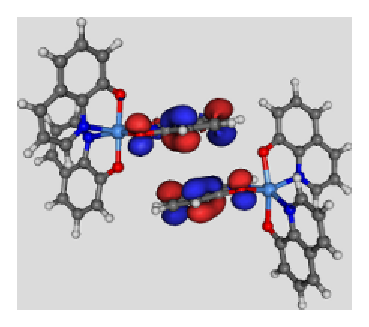
\includegraphics[width=17pt]{fig/logo_trans}}
\newcommand\votcacommand[2]
{
\begin{bclogo}[couleur=mygray, arrondi =0 , logo=\votcalogo, barre=line,noborder=true]{\small #1}
\itshape {\small #2}
\end{bclogo}
}

\newcommand\attention[1]
{
\begin{bclogo}[couleur=mygray, arrondi =0.1 , logo=\bctakecare, barre=line]{\small Be careful!}
{\small #1}
\end{bclogo}
}

\newcommand{\xml}{XML\xspace}
\newcommand{\gromacs}{\texttt{GROMACS}\xspace}
\newcommand{\gaussian}{\texttt{Gaussian}\xspace}
\newcommand{\turbomole}{\texttt{Turbomole}\xspace}
\newcommand{\nwchem}{\texttt{NWChem}\xspace}
\newcommand{\tinker}{\texttt{TINKER}\xspace}
\newcommand{\dipro}{\texttt{DIPRO}\xspace}

\newcommand{\Alq}{$\mathrm{Alq}_3$\xspace}
\newcommand{\dcvt}{DCV2T\xspace}

\newcommand{\xyz}{\texttt{geometry.xyz}\xspace}
\newcommand{\orb}{\texttt{zindo.orb}\xspace}
\newcommand{\votcaxtp}{{\MakeUppercase{votca-xtp}}\xspace}

\newcommand{\calculator}{\hyperref[sec:calculators]{calculator}\xspace}
\newcommand{\tool}{\hyperref[sec:calculators]{tool}\xspace}

\newcommand{\xmloptions}{\texttt{options.xml}\xspace}
\newcommand{\xmlcsg}{\hyperref[sec:xmlmap]{\texttt{map.xml}}\xspace}
\newcommand{\xmlsegments}{\hyperref[sec:xmlsegments]{\texttt{segments.xml}}\xspace}
\newcommand{\sqlstate}{\hyperref[sec:statefile]{\texttt{state.sql}}\xspace}
\newcommand{\sqlstateref}{\hyperref[sec:statefile]{\texttt{state\_ref.sql}}\xspace}
\newcommand{\sqlstatecg}{\hyperref[sec:statefile]{\texttt{state\_cg.sql}}\xspace}
\newcommand{\topology}{\texttt{topol.tpr}\xspace}
\newcommand{\trajectory}{\texttt{traj.xtc}\xspace}

\newcommand{\opt}{\texttt{{ -}o}\xspace}
\newcommand{\seg}{\texttt{{ -}s}\xspace}
\newcommand{\sql}{\texttt{{ -}f}\xspace}
\newcommand{\exe}{\texttt{{ -}e}\xspace}
\newcommand{\tpl}{\texttt{{ -}t}\xspace}
\newcommand{\csg}{\texttt{{ -}m}\xspace}
\newcommand{\trj}{\texttt{{ -}c}\xspace}
\newcommand{\job}{\texttt{{ -}j}\xspace}
\newcommand{\run}{\texttt{{run}}\xspace}
\newcommand{\wrt}{\texttt{{write}}\xspace}
\newcommand{\rd}{\texttt{{read}}\xspace}


\newcommand{\refcalc}{\hyperref[ref:calculators]{calculators}\xspace}

\newcommand{\overlap}{\hyperref[prog:xtp_overlap]{\texttt{xtp\_overlap}}\xspace}
\newcommand{\xtprun}{\hyperref[prog:xtp_run]{\texttt{xtp\_run}}\xspace}
\newcommand{\xtpmap}{\hyperref[prog:xtp_map]{\texttt{xtp\_map}}\xspace}
\newcommand{\xtpdipro}{\hyperref[prog:xtp_dipro]{\texttt{xtp\_dipro}}\xspace}
\newcommand{\xtpparallel}{\hyperref[prog:xtp_parallel]{\texttt{xtp\_parallel}}\xspace}
\newcommand{\xtpdump}{\hyperref[prog:xtp_dump]{\texttt{xtp\_dump}}\xspace}
\newcommand{\xtpupdate}{\hyperref[prog:xtp_update]{\texttt{xtp\_update}}\xspace}
\newcommand{\xtptools}{\hyperref[prog:xtp_tools]{\texttt{xtp\_tools}}\xspace}
\newcommand{\kmcrun}{\hyperref[prog:xtp_kmc_run]{\texttt{xtp\_kmc\_run}}\xspace}

\newcommand{\sqlite}{\texttt{sqlite3}\xspace}
\newcommand{\sqlconjsegproperties}{\texttt{conjseg\_properties}\xspace}
\newcommand{\sqlconjsegs}{\texttt{conjsegs}\xspace}
\newcommand{\sqlmolecules}{\texttt{molecules}\xspace}
\newcommand{\sqlpairintegrals}{\texttt{pairintegrals}\xspace}
\newcommand{\sqlpairproperties}{\texttt{pairproperties}\xspace}
\newcommand{\sqlpairs}{\texttt{pairs}\xspace}
\newcommand{\sqlrigidfragproperties}{\texttt{rigidfrag\_properties}\xspace}
\newcommand{\sqlrigidfrags}{\texttt{rigidfrags}\xspace}
\newcommand{\sqlframes}{\texttt{frames}\xspace}


\newcommand{\suggestion}[1]{{\color{red}SUGGESTION: #1}}

\newcommand{\segmentref}[1]{segments.#1}
\newcommand{\segmentopt}[1]{\hyperlink{\segmentref{#1}}{\StrSubstitute{#1}{_}{\_}}\xspace}
\newcommand{\calcref}[1]{#1}
\newcommand{\calcopt}[1]{\hyperlink{\calcref{#1}}{\StrSubstitute{#1}{_}{\_}}\xspace}

\newcommand{\calc}[1]{\hyperref[calc:#1]{\texttt{#1}}\xspace}
\newcommand{\toolref}[1]{\hyperref[tool:#1]{\texttt{#1}}\xspace}

\def\bibsection{%
    \chapter*{Bibliography}%
    \addcontentsline{toc}{chapter}{Bibliography}
}

\renewcommand*{\showkeyslabelformat}[1]{{\normalfont\tiny\sffamily#1}}
\definecolor{refkey}{rgb}{1,0,0}
\definecolor{labelkey}{rgb}{1,0,0}

% Calculus and Linear Algbra Notation
% formulas
\newcommand{\vctr}[1]{\mathbf{ \bar{#1} }}
\newcommand{\oper}[1]{\hat{ #1 }}
\newcommand{\matr}[1]{\mathbf{ #1 }}

%% FULL COMMANDS LISTING
\newcommand{\cmdmap}{\xtpmap \tpl \topology \trj \trajectory \seg \xmlcsg  \sql \sqlstate}
\newcommand{\cmdnbl}{\xtprun \opt \xmloptions  \sql  \sqlstate \exe  \calc{neighborlist}}
\newcommand{\cmdemlt}{\xtprun \opt \xmloptions  \sql  \sqlstate \exe  \calc{emultipole}}
\newcommand{\cmdeint}{\xtprun \opt \xmloptions  \sql  \sqlstate \exe  \calc{einternal}}
\newcommand{\cmdedft}{\xtpparallel \opt \xmloptions \sql \sqlstate \exe \calc{edft}}
\newcommand{\cmdidft}{\xtpparallel \opt \xmloptions \sql \sqlstate \exe \calc{idft}}
\newcommand{\cmdizindo}{\xtprun \opt \xmloptions  \sql  \sqlstate \exe  \calc{izindo}}
\newcommand{\cmdouter}{\xtprun \opt \xmloptions  \sql  \sqlstate \exe  \calc{outersphere}}
\newcommand{\cmdrates}{\xtprun \opt \xmloptions  \sql  \sqlstate \exe  \calc{rates}}
\newcommand{\cmdkmc}{ \kmcrun \opt \xmloptions  \sql  \sqlstate \exe  \calc{kmcmultiple}}
\newcommand{\cmdkmcsin}{ \kmcrun \opt \xmloptions  \sql  \sqlstate \exe  \calc{kmcsingle}}
\newcommand{\cmdeana}{\xtprun \opt \xmloptions  \sql  \sqlstate \exe  \calc{eanalyze}}
\newcommand{\cmdmolpol}{\xtptools \opt \xmloptions \exe \toolref{molpol}}
\newcommand{\cmdlogmps}{\xtptools \opt \xmloptions \exe \toolref{log2mps}}
\newcommand{\cmdxqmult}{\xtpparallel \opt \xmloptions \sql \sqlstate \exe \calc{xqmultipole}}
\newcommand{\cmdpanalyze}{ \xtprun \opt \xmloptions  \sql  \sqlstateref \exe  \calc{panalyze}}
\newcommand{\cmdeanast}{\xtprun \opt \xmloptions  \sql  \sqlstateref \exe  \calc{eanalyze}}
\newcommand{\cmdianalyze}{ \xtprun \opt \xmloptions  \sql  \sqlstateref \exe  \calc{ianalyze}}
\newcommand{\cmdnblst}{\xtprun \opt \xmloptions  \sql  \sqlstatecg \exe  \calc{neighborlist}}
\newcommand{\cmdeimport}{ \xtprun \opt \xmloptions  \sql  \sqlstateref \exe  \calc{eimport}}
\newcommand{\cmdiimport}{ \xtprun \opt \xmloptions  \sql  \sqlstatecg \exe  \calc{iimport}}
\newcommand{\cmdratesst}{\xtprun \opt \xmloptions  \sql  \sqlstatecg \exe  \calc{rates}}




\begin{document}

\addtolength{\oddsidemargin}{0cm}
\addtolength{\evensidemargin}{0cm}
\addtolength{\textwidth}{0cm}
\addtolength{\topmargin}{0cm}
\addtolength{\textheight}{0cm}




\lstdefinelanguage{XML2}
{
  morestring=[b]",
  morestring=[s]{>}{<},
  morecomment=[s]{<?}{?>},
  stringstyle=\color{black},
  identifierstyle=\color{darkblue},
  keywordstyle=\color{cyan},
  morekeywords={xmlns,version,type}% list your attributes here
}


\lstset{
  language=XML,
  frame=lines,
  backgroundcolor=\color{invisiblegray},
  basicstyle=\ttfamily\footnotesize,
  identifierstyle=\color{red},
  keywordstyle=\color{blue},
  commentstyle=\color{gray}\rmfamily\itshape,
  mathescape=false
}
\lstset{language=Python, 
        basicstyle=\ttfamily\small, 
        keywordstyle=\color{keywords},
        commentstyle=\color{comments},
        stringstyle=\color{red},
        showstringspaces=false,
        identifierstyle=\color{green}}


\setlength\parindent{0pt}
\frontmatter
\begin{titlepage}

%\center{\fontsize{4cm}{5cm}\selectfont VOTCA-CT}
%\center{\fontsize{1.5cm}{3cm}\selectfont USER MANUAL}

\center{\huge \sc VOTCA-XTP \\ \vspace*{1cm} Exciton Transport Simulations}
\vspace*{1cm}
\center{\Large \sc User Manual}

\vspace*{3cm}
\center{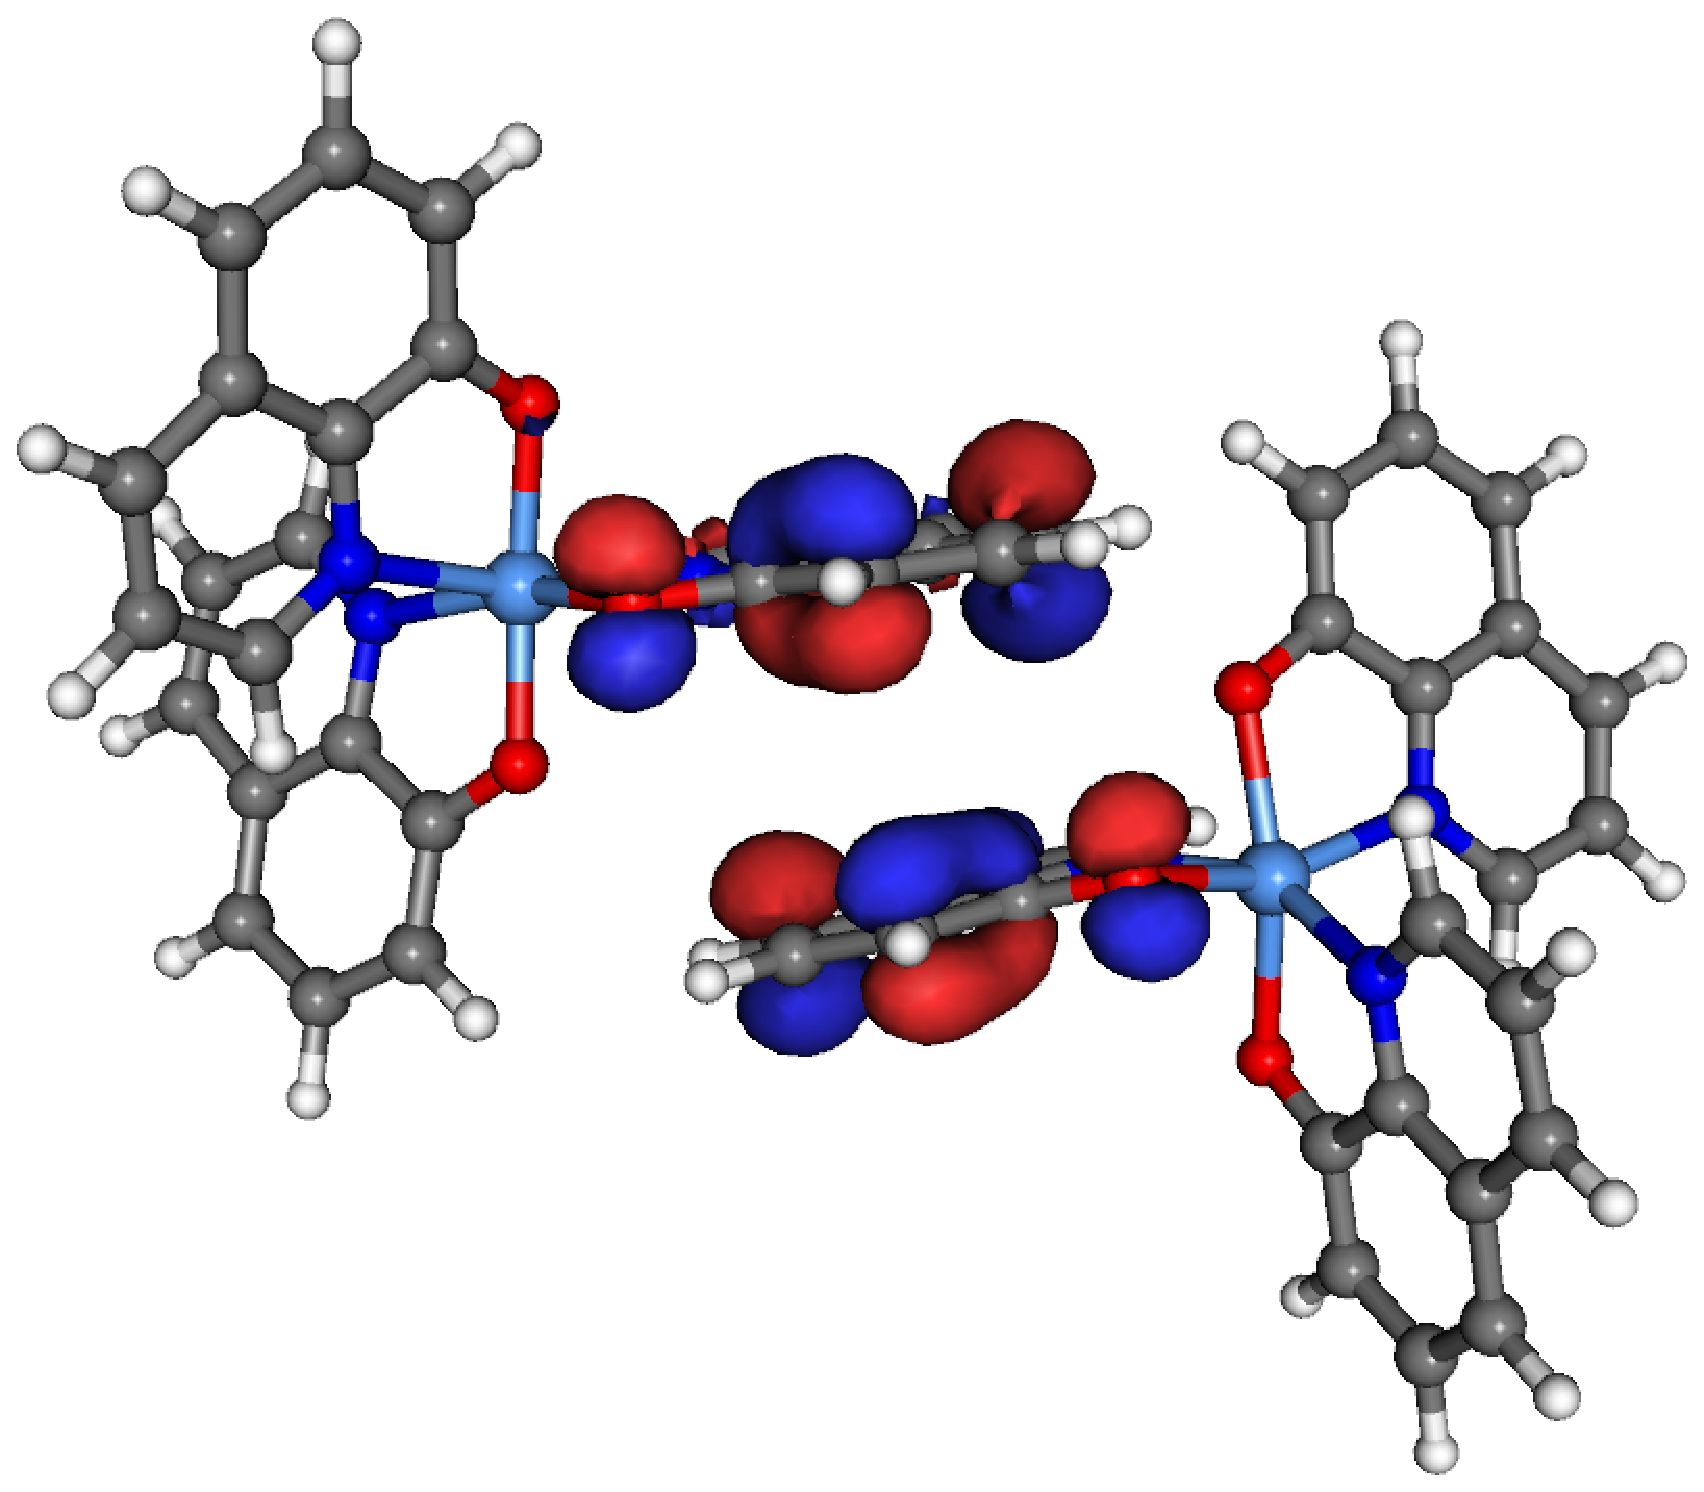
\includegraphics[width=0.6\columnwidth]{fig/logo}}
\vspace*{1cm}
\vfill

\center{\footnotesize{compiled from: \gitid}}
%\vspace*{1cm}
%\center{
%\large{\copyright \hspace*{0.1cm} VOTCA development team}
%}
\vspace*{0.5cm}
\center{\large{\today}} \\
\vspace*{0.3cm}
\htmladdnormallink{\color{black}\large{www.votca.org}}{http://www.votca.org}
\end{titlepage}

\section*{Disclamer}
This manual is still a very early version and thus not even clos to complete. If 
you need help, for each calculator the xml files are provided in the /share 
folder. Additonally the github page 
, the mailing list and the slack channel are useful to contact us. 
The reference section is generated automatically from the source code, so please 
make sure that your software and manual versions match.  

\section*{Citations}
Development of this software depends on academic research grants. If you are 
using the package, please cite the  following papers \\

\vspace{0.1cm}
\noindent
\cite{ruhle_microscopic_2011} Microscopic simulations of charge transport in 
disordered organic semiconductors, \\
Victor R\"uhle, Alexander Lukyanov, Falk May, Manuel Schrader, Thorsten Vehoff, 
James Kirkpatrick, Bj\"orn Baumeier and Denis Andrienko \\
\htmladdnormallink{  {\itshape J. Chem. Theor. Comp.} 7, 3335, 2011}
{http://dx.doi.org/10.1021/ct200388s} \\

\vspace{0.1cm}
\noindent
\cite{ruhle_versatile_2009} Versatile Object-oriented Toolkit for 
Coarse-graining Applications \\
Victor R\"uhle, Christoph Junghans, Alexander Lukyanov, Kurt Kremer and Denis 
Andrienko \\
\htmladdnormallink{  {\itshape J. Chem. Theor. Comp.} 5, 3211, 2009}
{http://dx.doi.org/10.1021/ct900369w}

\section*{Development}
The core development is currently taking place at the TU/e Eindhoven.

\section*{Copyright}
\votcaxtp is free software. The entire package is available under the Apache 
License. For details, check
the LICENSE file in the source code. The \votcaxtp source code is available on 
our homepage, 
\htmladdnormallink{\color{black}www.votca.org}{http://www.votca.org}.

\vfill

\thispagestyle{empty}
\cleardoublepage

\tableofcontents
\cleardoublepage
\mainmatter

\printindex
\vfill

\linenumbers

\chapter{Introduction}
\label{sec:introduction}

Charge carrier dynamics in an organic semiconductor can often be described in terms of charge hopping between localized states. The hopping rates depend on \slink{sec:transfer_integrals}{electronic coupling elements}, \slink{sec:reorganization}{reorganization energies}, and \slink{sec:site_energies}{site energies}, which vary as a function of position and orientation of the molecules. 
%The exact evaluation of these contributions in a molecular assembly is computationally prohibitive. Various, often semi-empirical, approximations are employed instead. 
The purpose of the \votcaxtp package~\cite{ruhle_microscopic_2011} is to simplify the workflow for charge transport simulations, provide a uniform error-control for the methods, flexible platform for their development, and eventually allow {\em in silico} prescreening of organic semiconductors for specific applications. 

The toolkit is implemented using modular concepts introduced earlier in the Versatile Object-oriented Toolkit for Coarse-graining Applications (VOTCA)~\cite{ruhle_versatile_2009}. It contains different \slink{sec:programs}{programs}, which execute specific tasks implemented in \slink{sec:calculators}{calculators} representing an individual step in the workflow. \Fig{summary} summarizes a typical chain of commands to perform a charge transport simulation:   
%
First, the VOTCA code structures are adap\-ted to reading atomistic trajectories, mapping them onto \slink{segments}{conjugated segments and rigid fragments}, and substituting (if needed) rigid fragments with the optimized copies (\xtpmap). The programs \xtprun and \xtpparallel (for heavy-duty tasks) are then used to calculate all bimolecular charge hopping rates (via precalculation of all required ingredients). \slink{sec:site_energies}{Site energies (or energetic disorder)} can be determined as a combination of internal (ionization potentials/electron affinities of single molecules) as well as electrostatic and polarization contributions within the molecular environment. The calculation of \slink{sec:transfer_integrals}{electronic coupling elements} between conjugated segments from the corresponding molecular orbitals can be performed using a \slink{sec:dipro}{dimer-projection} technique based on \slink{sec:dft}{density-functional} theory (DFT). This requires explicit calculations using quantum-chemistry software for which we provide interfaces to \gaussian, \turbomole, and \nwchem. Alternatively, the \slink{sec:izindo}{molecular orbital overlap} module calculates electronic coupling elements relying on the semi-empirical INDO Hamiltonian and molecular orbitals in the format provided by the \gaussian package. 

The  \slink{sec:kmc}{kinetic Monte Carlo} module reads in the \slink{neighborlist}{neighbor list}, \slink{morphology}{site coordinates}, and \slink{rates}{hopping rates} and performs charge dynamics simulations using either periodic boundary conditions or charge sources and sinks. 

The toolkit is written as a combination of modular C++ code and scripts. The data transfer between programs is implemented via a \slink{statefile}{state file} (sql database), which is also used to restart simulations. Analysis functions and most of the calculation routines are encapsulated by using the observer pattern~\cite{gamma_design_1995} which allows the implementation of new functions as individual modules.

In the following \sect{theory}, we summarize the \slink{sec:theory}{theoretical background} of the workflow of charge transport simulations and in particular its individual steps. \Sect{io} describes the structure and content of input and output files, while a full reference of \slink{sec:programs}{programs} and \slink{sec:calculators}{calculators} is available in \sect{reference}. For a hands-on tutorial, the reader is referred to the \hyperref[http://code.google.com/p/votca-xtp/]{\votcaxtp} project page at http://code.google.com/p/votca-xtp/.



\tikzstyle{decision} = [diamond, draw, fill=mygray]
\tikzstyle{line} = [draw, -stealth, thick]
\tikzstyle{block} = [draw, rectangle, fill=mygray, text width=0.5\linewidth]
\tikzstyle{smallblock} = [draw, rectangle, fill=mygray, text width=0.4\linewidth]
\tikzstyle{info} = [text width=0.35\linewidth]
\tikzstyle{smallinfo} = [text width=0.25\linewidth]
\tikzstyle{biginfo} = [text width=0.9\linewidth]
\begin{figure}
\centering
\newcommand{\vgap}{0.5cm}
\begin{scriptsize}
\noindent\begin{tikzpicture}
\node [block] (mapping) {{\bf Mapping}\\Converts and partitions atomistic \gromacs trajectory \vskip 0.1cm
{\noindent  \cmdmap}
\vskip 0.1cm};

\node[smallinfo, left=0.0 of mapping] (input) {{\bf Input files:}\\\texttt{conf.gro}\\\,\hskip 0.1cm\gromacs trajectory\\\texttt{topol.tpr}\\\hskip0.1cm\gromacs topology\\\texttt{\xmlcsg}\\\hskip0.1cm mapping and energies\\\texttt{options.xml}\\\hskip0.1cm options for \slink{sec:calculators}{calculators}\vskip 0.2cm {\bf Output files:}\\\texttt{\sqlstate}\\\hskip0.1cm \sqlite database file for\\\hskip0.1cm data transfer between\\\hskip0.1cm modules};

\node [block, below=\vgap of mapping] (nbl) {{\bf Neighbor list}\\Indentifies close molecular pairs between which charge transfer rates will be calculated \vskip 0.1cm
{\noindent \cmdnbl}
\vskip 0.1cm};


\node [block, below=\vgap of nbl] (site_energies) {{\bf Site energies}\\Calculates electrostatic and polarization contribution to site energies \vskip 0.1cm
{\noindent  \cmdemlt} };

\node [block, below=\vgap of site_energies] (int_energies) {{\bf Internal site and reorganization energies}\\Imports internal site energy (IP, EA) and reorganization energies for charging and discharging to \sqlstate \vskip 0.1cm
{\noindent  \cmdeint}
\vskip 0.1cm};


% above right=0.7cm and 4cm of A
\node[decision, below=\vgap of int_energies](decision1){Transfer integrals};

%\node (AuxNode01) [text width=6em, below of = decision1, node distance=7em ] {};

\node [smallblock, below left=\vgap of decision1] (DFT_TI) {{\bf Monomers with DFT}\\Calculate the relevant transport orbitals of monomers \vskip 0.1cm
{ \cmdedft \job\, ''\wrt \run'' }};

\node [smallblock, below=\vgap of DFT_TI] (DFT_TI2) {{\bf Transfer integrals with DFT}\\Calculate electronic coupling elements for all pairs in the neighbor list \vskip 0.1cm
{ \cmdidft \job\, ''\wrt \run \rd'' }
\vskip 0.1cm};

\node [smallblock, below right=\vgap of decision1] (DFT_ZINDO) {{\bf Transfer integrals with ZINDO}\\Calculate electronic coupling elements for all pairs in the neighbor list  \vskip 0.1cm
{\noindent  \cmdizindo }
\vskip 0.1cm};


\node[info, below=0.2cm of DFT_ZINDO] (ti_info) {{One can choose between quantum-chemical (computationally expensive) or semi-empirical (fast, but not always sufficiently accurate) evaluation of transfer integrals.}};

\node (AuxNode01) [below=\vgap of DFT_TI2, xshift=0.25\linewidth] {};


\node [block, below=\vgap of DFT_TI2, xshift=0.275\linewidth] (outer_reorg) {{\bf Outersphere reorganization energies}\\Contribution to reorganization of surrounding molecules due to polarization. (optional for Marcus rates)  \vskip 0.1cm
{\noindent  \cmdouter}
\vskip 0.1cm};

\node [block, below=\vgap of outer_reorg] (rates) {{\bf Charge transfer rates}\\Calculates rates for charge transfer among all pairs in the neighborlist \vskip 0.1cm
{\noindent \cmdrates}
};

\node [block, below=\vgap of rates] (kmc) {{\bf Charge dynamics via kMC}\\Hopping of charge carriers simulated via kinetic Monte Carlo \vskip 0.1cm
{\noindent \cmdkmc }
};

\node [biginfo, below=\vgap of kmc] (calc) {{\noindent Get list of available calculators: \xtprun/\xtpparallel/\kmcrun  \texttt{ -l}}\\ Get help and list of options for a calculator: \xtprun/\xtpparallel/\kmcrun  \texttt{ -d }\calc{neighborlist}};

\path [line] (mapping) -- (nbl);
\path [line] (nbl) -- (site_energies);
\path [line] (site_energies) -- (int_energies);
\path [line] (int_energies) -- (decision1);
\path [line] (DFT_TI) -- (DFT_TI2);
\path [line] (decision1) -| node[yshift=0.5em, xshift=1em] {DFT} (DFT_TI);
\path [line] (decision1) -| node[yshift=0.5em, xshift=-1em] {ZINDO} (DFT_ZINDO);
\path [line] (DFT_TI2.east) -| (outer_reorg.north);
\path [line] (DFT_ZINDO.west) -| (outer_reorg);
\path [line] (outer_reorg) -- (rates);
\path [line] (rates) -- (kmc);
\end{tikzpicture}


\end{scriptsize}
\caption{A practical workflow of charge transport simulations using \votcaxtp. The \slink{sec:theory}{theoretical background} of the individual steps is given in \sect{theory}. \Sect{io} describes the content of input and output files, while a full reference of \slink{sec:programs}{programs} and \slink{sec:calculators}{calculators} is available in \sect{reference}.  }
\label{fig:summary}
\end{figure}


\chapter{Theoretical background}
\label{sec:theory}

\section{Workflow}
\label{sec:wokflow}

A typical workflow of charge transport simulations is depicted in \fig{workflow}. The first step is the simulation of an \slink{morphology}{atomistic morphology}, which is then partitioned on \slink{segments}{hopping sites}. The coordinates of the hopping sites are used to construct a list of pairs of molecules, or \slink{neighborlist}{neighbor list}. 

\begin{figure}[h]
   \label{fig:workflow}
\includegraphics[width=\textwidth]{fig/workflow/workflow}
 \caption{%
   Workflow for microscopic simulations of charge transport.  %
}
\end{figure}

For each pair an \slink{transfer_integrals}{electronic coupling element}, a \slink{reorganization}{reorganization energy}, a \slink{site_energies}{driving force}, and eventually the \slink{rates}{hopping rate} are evaluated. The neighbor list and hopping rates define a directed graph. The corresponding master equation is solved using the \slink{kmc}{kinetic Monte Carlo} method, which allows to explicitly monitor the charge dynamics in the system as well as to calculate time or ensemble averages of occupation probabilities, charge fluxes, correlation functions, and field-dependent mobilities.

% 
% \begin{figure}[p]
% \includegraphics[width=\textwidth]{fig/workflow_practical/workflow_practical}
%  \caption{%
%    Workflow for microscopic simulations of charge transport including calls.  %
%    \label{fig:workflow}}
% \end{figure}



	
\section{Material morphology}
\label{sec:morphology}

There is no generic recipe on how to predict a large-scale atomistically-resolved morphology of an organic semiconductor. The required methods are system-specific: for ultra-pure crystals, for example, density-functional methods can be used provided the crystal structure is known from experiment. For partially disordered organic semiconductors, however, system sizes much larger than a unit cell  are required. Classical molecular dynamics or Monte Carlo techniques are then the methods of choice. 

In molecular dynamics, atoms are represented by point masses which interact via empirical potentials prescribed by a force-field. Force-fields are parametrized for a limited set of compounds and their refinement is often required for new molecules. In particular, special attention shall be paid to torsion potentials between successive repeat units of conjugated polymers or between functional groups and the $\pi$-conjugated system. First-principles methods can be used to characterize the missing terms of the potential energy function. 

Self-assembling materials, such as soluble oligomers, discotic liquid crystals, block copolymers, partially crystalline polymers, etc., are the most complicated to study. The morphology of such systems often has several characteristic length scales and can be kinetically arrested in a thermodynamically non-equilibrium state. For such systems, the time- and length-scales of atomistic simulations might be insufficient to equilibrate or sample desired morphologies. In this case, systematic coarse-graining can be used to enhance sampling~\cite{ruhle_versatile_2009}. Note that the coarse-grained representation must reflect the structure of the atomistic system and allow for back-mapping to the atomistic resolution.

Here we assume that the morphology is already known, that is we know how the topology and the coordinates of all atoms in the systems at a given time. \votcaxtp can read standard \gromacs topology files. Custom definitions of \slink{sec:atomistic}{atomistic topology} via \xml files are also possible. Since the description of the atomistic topology is the first step in the charge transport simulations, it is important to follow simple conventions on how the system is partitioned on molecules, residues, and how atoms are named in the topology. Required input files are described in section \slink{sec:atomistic}{atomistic topology}. 

\section{Conjugated segments and rigid fragments}
\label{sec:segments}

\begin{figure}
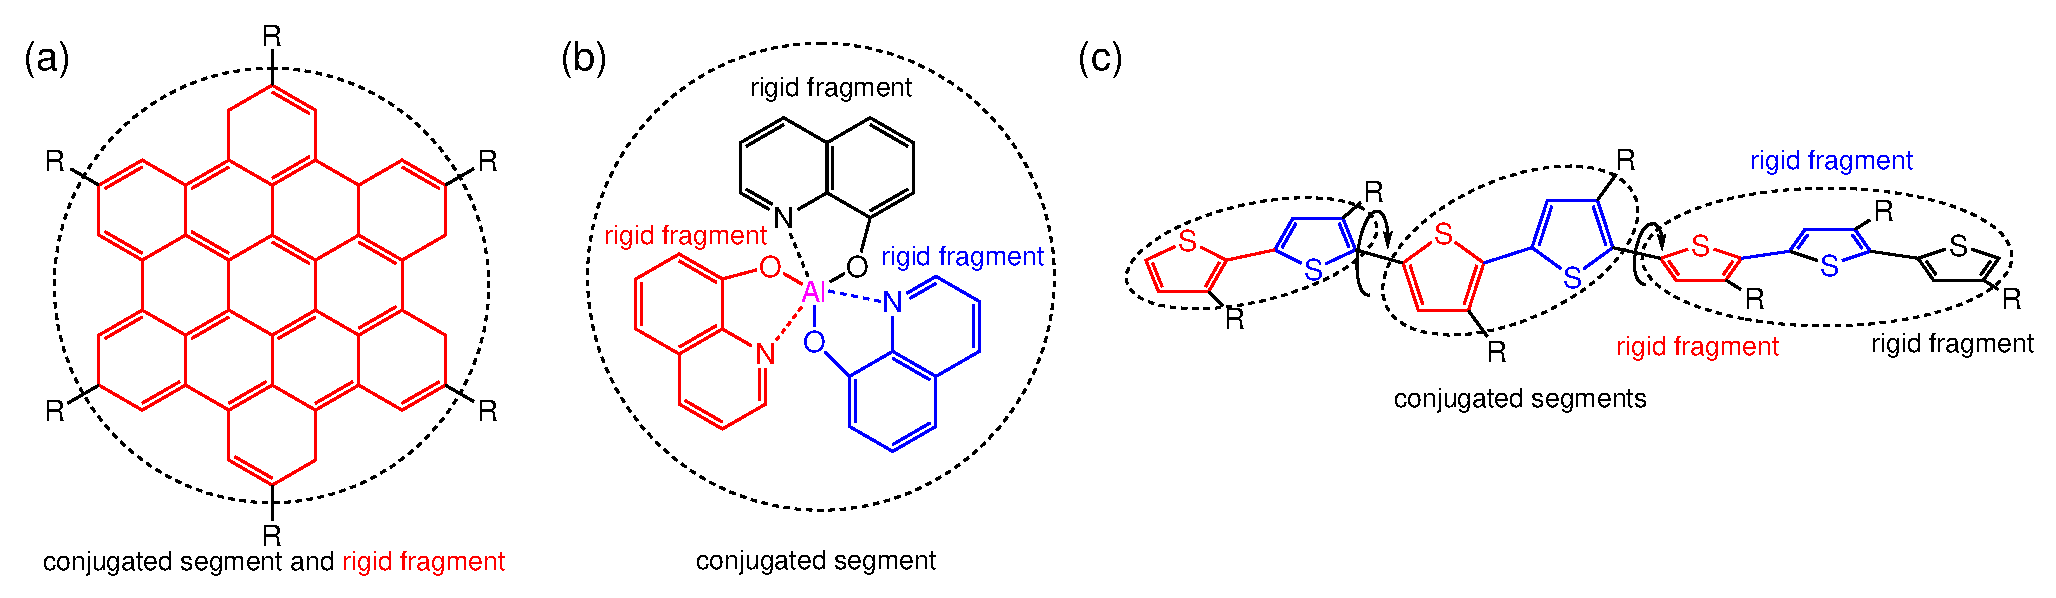
\includegraphics[width=\linewidth]{fig/conjugated_segment/fragment_segment}
\caption{The concept of conjugated segments and rigid fragments. Dashed lines indicate conjugated segments while colors denote rigid fragments. (a) Hexabenzocoronene: the $\pi$-conjugated system is both a rigid fragment and a conjugated segment. (b) \Alq: the Al atom and each ligand are rigid fragments while the whole molecule is a conjugated segment. (c) Polythiophene: each repeat unit is a rigid fragment. A conjugated segment consists of one or more rigid fragments. One molecule can have several conjugated segments.}
\label{fig:segment}
\end{figure}

With the morphology at hand, the next step is partitioning the system on hopping sites\index{hopping site}, or conjugated segments\index{conjugated segment}, and calculating charge transfer rates between them. Physically intuitive arguments can be used for the partitioning,  which reflects the localization of the wave function of a charge. For most organic semiconductors, the molecular architecture includes relatively rigid, planar $\pi$-conjugated systems, which we will refer to as rigid fragments. A conjugated segment can contain one or more of such rigid fragments, which are linked by bonded degrees of freedom. The dynamics of these degrees of freedom evolves on timescales much slower than the frequency of the internal promoting mode. In some cases, e.g. glasses, it can be `frozen' due to non-bonded interactions with the surrounding molecules.

To illustrate the concept of conjugated segments and rigid fragments, three representative molecular architectures are shown in \fig{segment}. The first one is a typical discotic liquid crystal, hexabenzocoronene. It consists of a conjugated core to which side chains are attached to aid self-assembly and solution processing. In this case the orbitals localized on side chains do not participate in charge transport and the conjugated $\pi$-system is both, a rigid fragment and a conjugated segment. 
%
In \Alq, a metal-coordinated compound, a charge carrier is delocalized over all three ligands. Hence, the whole molecule is one conjugated segment. Individual ligands are relatively rigid, while energies of the order of $k_\text{B}T$ are sufficient to reorient them with respect to each other. Thus the Al atom and the three ligands are rigid fragments.
%
In the case of a conjugated polymer, one molecule can consist of several conjugated segments, while each backbone repeat unit is a rigid fragment. Since the conjugation along the backbone can be broken due to large out-of-plane twists between two repeat units, an empirical criterion, based on the dihedral angle, can be used to partition the backbone on conjugated segments~\cite{ruhle_multiscale_2010}. However, such intuitive partitioning is, to some extent, arbitrary and shall be validated by other methods~\cite{vukmirovic_charge_2008,vukmirovic_charge_2009,mcmahon_ad_2009}. 

After partitioning, an additional step is often required to remove bond length fluctuations introduced by molecular dynamics simulations, since they are already integrated out in the derivation of the rate expression. This is achieved by substituting respective molecular fragments with  rigid, planar $\pi$-systems\index{rigid fragment} optimized using first-principles methods. Centers of mass and gyration tensors are used to align rigid fragments, though a custom definition of local axes is also possible. Such a procedure also minimizes discrepancies between the force-field and first-principles-based ground state geometries of conjugated segments, which might be important for calculations of electronic couplings, reorganization energies, and intramolecular driving forces. 

To partition the system on hopping sites and substitute rigid fragments with the corresponding ground-state geometries \xtpmap program is used:
\votcacommand{Mapping the \gromacs trajectory}{\cmdmap}
It reads in the \gromacs topology (\topology) and trajectory (\trajectory) files, definitions of conjugated segments and rigid fragments (\xmlcsg) and outputs coordinates of conjugated segments (hopping sites) and rigid fragments (as provided in the MD trajectory and after rigidification) to the  state file (\sqlstate). In order to do this, a mapping file \xmlcsg has to be provided, which specifies the corresponding atoms in the different representations. After this step, all information (frame number, dimensions of the simulation box, etc) are stored in the \slink{statefile}{state file} and only this file is used for further calculations.

\attention{\votcaxtp requires a wrapped trajectory for mapping the segments and fragments, so all molecules should be whole in the frame.}   

In order to visually check the mapping one can use either the \calc{tdump} \calculator or the programm \xtpdump with the calculator \calc{trajectory2pdb}.

\label{sec:xtp_dump}
\votcacommand{Writing a mapped trajectroy with \xtpdump}{\small \xtpdump \sql \sqlstate \exe \calc{trajectory2pdb} }

It reads in the state file created by \xtpmap and outputs two trajectory files corresponding to the original and rigidified atom coordinates. To check the mapping, it is useful to superimpose the three outputs (original atomistic, atomistic stored in the state file, and rigidified according to ground state geometries), e.g., with {\tt VMD}.

\label{sec:tdump}
\votcacommand{Writing a mapped trajectroy with \calc{tdump} }{\small \xtprun \sql \sqlstate \opt \xmloptions \exe \calc{tdump} }

It also reads in the state file but appends the coordinates to a pdb. file. So make sure to delete old QM.pdb and MD.pdb if you want to create a new imagef



\section{Neighbor list}
\label{sec:neighborlist}

A list of neigboring conjugated segments, or neighbor list\index{neighbor list}, contains all pairs of conjugated segments for which \slink{sec:transfer_integrals}{coupling elements}, \slink{sec:reorganization}{reorganization energies}, \slink{sec:site_energies}{site energy differences}, and \slink{sec:rates}{rates} are evaluated.

Two segments are added to this list if the distance between centers of mass of any of their rigid fragments is below a certain cutoff. This allows neighbors to be selected on a criterion of minimum distance of approach rather than center of mass distance, which is useful for molecules with anisotropic shapes.

The neighbor list can be generated from the atomistic trajectory by using the \calc{neighborlist} \calculator. This calculator requires a cutoff, which can be specified in the \xmloptions file. The list is saved to the \sqlstate file:
\votcacommand{Generating a neighbor list}{\cmdnbl}

\section{Reorganization energy}
\label{sec:reorganization}

The reorganization energy\index{reorganization energy} $\lambda_{ij}$ takes into account the change in  nuclear (and dielectric) degrees of freedom as the charge moves from donor $i$ to acceptor $j$. It has two contributions: intramolecular, $\lambda^\text{int}_{ij}$, which is due to reorganization of nuclear coordinates of the two molecules forming the charge transfer complex, and intermolecular (outersphere), $\lambda^\text{out}_{ij}$, which is due to the relaxation of the nuclear coordinates of the environment. In what follows we discuss how these contributions can be calculated.

\subsection{Intramolecular reorganization energy}
\label{sec:eintramolecular}
\index{reorganization energy!intramolecular}
If intramolecular vibrational modes of the two molecules are treated classically, the rearrangement of their nuclear coordinates after charge transfer results in the dissipation of the internal reorganization energy, $\lambda_{ij}^\text{int}$. It can be computed from four points on the potential energy surfaces (PES) of both molecules in neutral and charged states, as indicated in \fig{parabolas}. 

\begin{figure}
   \centering
   \includegraphics[width=0.6\linewidth]{fig/reorganization_energy/monomer_parabolas}
    \caption{Potential energy surfaces of (a) donor and (b) acceptor in charged and neutral states. After the change of the charge state both molecules relax their nuclear coordinates. If all vibrational modes are treated classically, the total internal reorganization energy and the internal energy difference of the electron transfer reaction are $\lambda_{ij}^\text{int} = \lambda_{i}^{cn} + \lambda_{j}^{nc}$ and $\Delta E_{ij}^\text{int} =  \Delta U_i - \Delta U_j$, respectively.}
   \label{fig:parabolas}
\end{figure}


Adding the contributions due to discharging of molecule $i$ and charging of molecule $j$ yields~\cite{bredas_charge-transfer_2004}
\begin{equation}
\lambda_{ij}^\text{int} =\lambda_{i}^{cn}+\lambda_{j}^{nc}=U_{i}^{nC}-U_{i}^{nN}+U_{j}^{cN}-U_{j}^{cC}\,.
\label{equ:lambdas}
\end{equation}
Here $U_{i}^{nC}$ is the internal energy of the neutral molecule $i$ in the geometry of its charged state (small $n$ denotes the state and capital $C$ the geometry). Similarly, $U_{j}^{cN}$ is the energy of the charged molecule $j$ in  the geometry of its neutral state.
%If the PES of neutral and charged states are different for the same molecule, that is  $\lambda^{cn}_i \neq \lambda^{nc}_i$, the rate for the bimolecular charge transfer is no longer a simple sum. If, as before, both modes are treated classically, the rate is an integral over the charge detachment and attachment spectrum of molecules $i$ and $j$~\cite{kakitani_comprehensive_1987}. For most systems, however, the reorganization energies for charging or discharging of the same molecule do not deviate by more than a few percent and the rate is given by~\equ{marcus}.
%
Note that the PES of the donor and acceptor are not identical for chemically different compounds or for conformers of the same molecule. In this case $\lambda_{i}^{cn} \ne \lambda_{j}^{cn}$ and  $\lambda_{i}^{nc} \ne \lambda_{j}^{nc}$. Thus $\lambda_{ij}^\text{int}$ is a property of the charge transfer complex, and not of a single molecule.

Intramolecular reorganization energies for discharging ($\lambda^{cn}$) and charging ($\lambda^{nc}$) of a molecule need to be determined using quantum-chemistry and given in \xmlcsg. The values are written to the \sqlstate using the calculator \calc{einternal} (see also \slink{sec:einternal}{internal energy}):
\votcacommand{Intramolecularl reorganization energies}{\cmdeint}

\subsection{Outersphere reorganization energy}
\index{reorganization energy!outersphere}
\label{sec:eoutersphere}
During the charge transfer reaction, also the molecules outside the charge transfer complex reorient and polarize in order to adjust for changes in electric potential, resulting in the outersphere contribution to the reorganization energy. $\lambda_{ij}^\text{out}$ is particularly important if charge transfer occurs in a polarizable environment. Assuming that charge transfer is much slower than electronic polarization but much faster than nuclear rearrangement of the environment, $\lambda_{ij}^\text{out}$ can be calculated from the electric displacement fields created by the charge transfer complex~\cite{may_relationship_2011}
\begin{equation}
\lambda_{ij}^\text{out}=
\frac{c_p}{2\epsilon_0}\int_{V^\text{out}}d V
\left[ \vec{D}_I(\vec{r}) - \vec{D}_F(\vec{r}) \right]^2\,,
\label{equ:lambda_outer1}
\end{equation}
where $\epsilon_0$ is the the permittivity of free space, $\vec{D}_{I,F}(\vec{r})$ are the electric displacement fields created by the charge transfer complex in the initial (charge on molecule $i$) and final (charge transferred to molecule $j$) states,  $V^\text{out}$ is the volume outside the complex, and $c_p=\frac{1}{\epsilon_\text{opt}}-\frac{1}{\epsilon_\text{s}}$ is the Pekar factor, which is determined by the low ($\epsilon_\text{s}$) and high ($\epsilon_\text{opt}$) frequency dielectric permittivities.

\Equ{lambda_outer1} can be simplified by assuming spherically symmetric charge distributions on molecules $i$ and $j$ with total charge $e$. Integration over the volume $V^\text{out}$ outside of the two spheres of radii $R_i$ and $R_j$ centered on molecules $i$ and $j$ leads to the classical Marcus expression for the outersphere reorganization energy
\begin{equation}
\lambda_{ij}^\text{out}=\frac{c_{p}e^2}{4\pi\epsilon_0}\left(\frac{1}{2 R_i}+\frac{1}{2 R_j}-\frac{1}{r_{ij}} \right)\,,
\label{equ:lambda_outer2}
\end{equation}
where $r_{ij}$ is the molecular separation.  While \equ{lambda_outer2} captures the main physics, e.g. predicts smaller outer-sphere reorganization energies (higher rates) for molecules at smaller separations, it often cannot provide quantitative estimates, since charge distributions are rarely spherically symmetric. 

Alternatively, the displacement fields can be constructed using the atomic partial charges. The difference of the displacement fields at the position of an atom $b_k$ outside the charge transfer complex (molecule $k \ne i,j$)  can be expressed as
\begin{eqnarray}
\label{equ:disp_atom}
\vec{D}_I(\vec{r}_{b_k}) - \vec{D}_F(\vec{r}_{b_k})  = 
\sum_{a_i} \frac{q_{a_i}^c - q_{a_i}^n}{4\pi } \frac{ (\vec{r}_{b_k} - \vec{r}_{a_i} ) }
                                            {|\vec{r}_{b_k}-\vec{r}_{a_i}|^3}+
\sum_{a_j} \frac{q_{a_j}^n - q_{a_j}^c}{4\pi } \frac{ (\vec{r}_{b_k}-\vec{r}_{a_j} ) } 
                                            {|\vec{r}_{b_k}-\vec{r}_{a_j}|^3}\,,
%\nonumber
\end{eqnarray}
where $q^n_{a_i}$ ($q^c_{a_i}$) is the partial charge of atom $a$ of the neutral (charged) molecule $i$ in vacuum. The partial charges of neutral and charged molecules are obtained by fitting their values to reproduce the electrostatic potential of a single molecule (charged or neutral) in vacuum. 
%
Assuming a uniform density of atoms, the integration in~\equ{lambda_outer1} can be rewritten as a density-weighted sum over all atoms excluding those of the charge transfer complex.

The remaining unknown needed to calculate $\lambda_{ij}^\text{out}$ is the Pekar factor\index{Pekar factor}, $c_p$. In polar solvents $\epsilon_\text{s}\gg\epsilon_\text{opt}\sim 1$ and $c_p$ is of the order of 1. In most organic semiconductors, however, molecular orientations are fixed and therefore the low frequency dielectric permittivity is of the same order of magnitude as $\epsilon_\text{opt}$. Hence, $c_p$ is small and its value is very sensitive to differences in the permittivities. 


Outersphere reorganization energies for all pairs of molecules in the \slink{sec:neighborlist}{neighbor list} can be computed from the atomistic trajectory by using the \calc{eoutersphere} \calculator. 

Two methods can be used to compute $\lambda_{ij}^\text{out}$. The first method uses the atomistic partial charges of neutral and charged molecules from files specified in \xmlcsg and \equ{lambda_outer1}. The Pekar factor $c_p$ and a cutoff radius  based on molecular centers of mass have to be specified in the \xmloptions file. 

If this method is computationally prohibitive, $\lambda_{ij}^\text{out}$ can be computed using \equ{lambda_outer2}, which assumes spherical charge distributions on the molecules. In this case the radii of these spheres are specified in \xmlsegments, while the Pekar factor $c_p$ is given in the \xmloptions file and no cutoff radius is needed. 

The outer sphere reorganization energies are saved to the \sqlstate file:
\votcacommand{Outersphere reorganization energy}{\cmdouter}

\section{Site energies}
\label{sec:site_energies}
A charge transfer reaction between molecules $i$ and $j$ is driven by the site 
energy\index{site energy} difference, $\Delta E_{ij} = E_i - E_j$. Since the  
transfer rate, $\omega_{ij}$, depends exponentially on $\Delta E_{ij}$ 
(see~\equ{marcus}) it is important to compute its distribution as accurately as 
possible.  The total site energy difference has contributions due to 
\slink{sec:ext_field}{externally applied electric field}, 
\slink{sec:ecoulomb}{electrostatic interactions}, polarization effects, and 
\slink{sec:internal_energy}{internal energy} differences. In what follows we 
discuss how to estimate these contributions by making use of first-principles 
calculations and polarizable force-fields.

\subsection{Externally applied electric field}
\label{sec:ext_field}
The contribution to the total site energy\index{site energy!external field} 
difference due to an external electric field $\vec{F}$ is given by $\Delta 
E_{ij}^\text{ext} = q {\vec{F} \cdot \vec{r}_{ij}}$, where $q=\pm e$ is the 
charge and $\vec{r}_{ij} = \vec{r}_i  - \vec{r}_j $ is a vector connecting 
molecules $i$ and $j$. For typical distances between small molecules, which are 
of the order  of $1\,\unit{nm}$, and moderate fields of $F<10^8\,\unit{V/m}$ 
this term is always smaller than $0.1\, \unit{eV}$.

\subsection{Internal energy}
\label{sec:internal_energy}

The contribution to the site energy difference due to different internal 
energies\index{site energy!internal} (see \fig{parabolas}) can be written as
\begin{equation}
 \Delta E_{ij}^\text{int}=
\Delta U_i - \Delta U_j = \left( U_{i}^{cC}-U_{i}^{nN}\right) - \left( 
U_{j}^{cC}-U_{j}^{nN}\right) \, ,
\label{equ:conformational}
\end{equation}
where $U_{i}^{cC(nN)}$ is the total energy of molecule $i$ in the charged 
(neutral) state and geometry.  $\Delta U_{i}$ corresponds to the adiabatic 
ionization potential (or electron affinity) of molecule $i$, as shown 
in~\fig{parabolas}. For one-component systems and negligible conformational 
changes $ \Delta E_{ij}^\text{int}=0$, while it is significant for 
donor-acceptor systems. 

Internal energies determined using quantum-chemistry need to be specified in 
\xmlmap. The values are written to the \sqlstate using the calculator 
\calc{einternal} (see also \slink{sec:eintramolecular}{intramolecular 
reorganization energy}):
\votcacommand{Internal energies}{\cmdeint}

\subsection{Induction energy - the Thole model}
\label{sec:thole_model}
\index{Thole model}
\index{site energy!polarization}


If we in addition to the permanent set of multipole moments $\{Q_t^a\}$ allow 
for induced moments $\{\Delta Q_t^a\}$ and penalize their generation with a 
bilinear form (giving rise to a strictly positive contribution to the energy),
\begin{align}
U_\textrm{int} &=\frac{1}{2} \sum_A \Delta Q_t^a \eta_{tt'}^{aa'} \Delta 
Q_{t'}^{a'},
\end{align}
it can be shown that the induction contribution to the site energy evaluates to 
an expression where all interactions between induced moments have cancelled out, 
and interactions between permanent and induced moments are scaled down by 
$1/2$~\cite{stone_theory_1997}:
\begin{align}
U_{pu} = \frac{1}{2} \sum_A \sum_{B > A} \left[ \Delta Q_t^a T_{tu}^{ab} Q_u^b + 
\Delta Q_t^b T_{tu}^{ab} Q_u^a \right].
\label{equ:u_pu}
\end{align}
This term can be viewed as the second-order (induction) correction to the 
molecular interaction energy. The sets of $\{Q_t^a\}$ are solved for 
self-consistently via
\begin{align}
\Delta Q_t^a = - \sum_{B \neq A} \alpha_{tt'}^{aa'} T_{t'u}^{a'b} (Q_u^b + 
\Delta Q_u^b),
\label{equ:self_consistent_dQ}
\end{align}
where the polarizability tensors $\alpha_{tt'}^{aa'}$ are given by the inverse 
of $\eta_{tt'}^{aa'}$.

With eqs.~\ref{equ:self_consistent_dQ} and~\ref{equ:u_pu} we have at hand 
expressions that allow us to compute the induction energy contribution to site 
energies in an iterative manner based on a set of molecular distributed 
multipoles $\{Q_t^a\}$ and polarizabilities $\{\alpha_{tt'}^{aa'}\}$. We have 
drafted in the previous section how to obtain the former from a wavefunction 
decomposition or fitting scheme (GDMA, CHELPG). The $\{\alpha_{tt'}^{aa'}\}$ can 
be derived formally (or rather: read off) from a perturbative expansion of the 
molecular interaction. In this work we make use of the Thole 
model~\cite{thole_molecular_1981, van_duijnen_molecular_1998} as a 
semi-empirical approach to obtain the sought-after point polarizabilities in the 
local dipole approximation, that is, $[\alpha_{tt'}^{aa'}] = \alpha_{tt'}^{aa'} 
\delta_{t \beta} \delta_{t'\beta} \delta_{aa'}$, where $\beta \epsilon 
\{x,y,z\}$ references the dipole-moment component.

The Thole model is based on a modified dipole-dipole interaction, which can be 
reformulated in terms of the interaction of smeared charge densities. This has 
been shown to be necessary due to the divergent head-to-tail dipole-dipole 
interaction that otherwise results at small interseparations on the 
\AA~scale~\cite{applequist_atom_1972, thole_molecular_1981, 
van_duijnen_molecular_1998}. Smearing out the charge distribution mimics the 
nature of the QM wavefunction, which effectively guards against this unphysical 
polarization catastrophe. Since the point dipoles however only react 
individually to the external field, any correlation effects as were still 
accounted for in the $\{\alpha_{tt'}^{aa'}\}$ are lost, except perhaps those 
correlations that are due to the mere classical field interaction.

The smearing of the nuclei-centered multipole moments is obtained via a 
fractional charge density $\rho_f(\vec{u})$ which should be normalized to unity 
and fall off rapidly as of a certain radius $\vec{u} = \vec{u}(\vec{R})$. The 
latter is related to the physical distance vector $\vec{R}$ connecting two 
interacting sites via a linear scaling factor that takes into account the 
magnitude of the isotropic site polarizabilities $\alpha^a$. This isotropic 
fractional charge density gives rise to a modified potential
\begin{align}
 \phi(u) = -\frac{1}{4\pi\varepsilon_0} \int \limits_{0}^{u} \! 4\pi u' \rho(u') 
d\!u' 
 \label{equ:mod_potential}
\end{align}
We can relate the multipole interaction tensor $T_{ij \dots}$ (this time in 
Cartesian coordinates) to the fractional charge density in two steps: First, we 
rewrite the tensor in terms of the scaled distance vector $\vec{u}$,
\begin{align}
 T_{ij \dots }(\vec{R}) = f(\alpha^a \alpha^b) \ t_{ij 
\dots}(\vec{u}(\vec{R},\alpha^a \alpha^b)),
\end{align}
where the specific form of $f(\alpha^a \alpha^b)$ results from the choice of 
$u(\vec{R},\alpha^a \alpha^b)$. Second, we demand that the smeared interaction 
tensor $t_{ij \dots}$ is given as usual by the appropriate derivative of the 
potential in eq.~\ref{equ:mod_potential},
\begin{align}
 t_{ij \dots}(\vec{u}) = - \partial_{u_i} \partial_{u_j} \dots \phi(\vec{u}).
\end{align}
It turns out that for a suitable choice of $\rho_f(\vec{u})$, the modified 
interaction tensors can be rewritten in such a way that powers $n$ of the 
distance $R = |\vec{R}|$ are damped with a damping function 
$\lambda_n(\vec{u}(\vec{R}))$~\cite{ren_polarizable_2003}.

There is a large number of fractional charge densities $\rho_f(\vec{u})$ that 
have been tested for the purpose of giving best results for the molecular 
polarizability as well as interaction energies. Note how a great advantage of 
the Thole model is the exceptional transferability of the atomic 
polarizabilities to compounds not used for the fitting 
procedure~\cite{van_duijnen_molecular_1998}. In fact, for most organic 
molecules, a fixed set of atomic polarizabilities ($\alpha_C = 1.334$, $\alpha_H 
= 0.496$, $\alpha_N = 1.073$, $\alpha_O = 0.873$, $\alpha_S = 2.926$ \AA$^3$) 
based on atomic elements yields satisfactory results.

VOTCA implements the Thole model with an exponentially-decaying fractional 
charge density
\begin{align}
 \rho(u) = \frac{3a}{4\pi} \exp(-au^3),
\end{align}
where $\vec{u}(\vec{R},\alpha^a \alpha^b) = \vec{R} / (\alpha^a \alpha^b)^{1/6}$ 
and the smearing exponent $a=0.39$ (which can however be changed from the 
program options), as used in the AMOEBA force field~\cite{ren_polarizable_2003}.

Even though the Thole model performs very well for many organic compounds with 
only the above small set of element-based polarizabilities, conjugated molecules 
may require a more intricate parametrization. The simplest approach is to resort 
to scaled polarizabilities to match the effective molecular polarizable volume 
$V \sim \alpha_{x} \alpha_{y} \alpha_{z}$ as predicted by QM calculations (here 
$\alpha_x, \alpha_y, \alpha_z$ are the eigenvalues of the molecular 
polarizability tensor). The \toolref{molpol} \tool assists with this task, it 
self-consistently calculates the Thole polarizability for an input mps-file and 
optimizes (if desired) the atomic polarizabilities in the above simple manner.

\votcacommand{Generate Thole-type polarizabilites for a segment}{\cmdmolpol}

The electrostatic and induction contribution to the site energy is evaluated by 
the \calc{emultipole} \calculator. Atomistic partial charges for charged and 
neutral molecules are taken from mps-files (extended GDMA format) specified in 
\xmlmap. Note that, in order to speed up calculations for both methods, a 
cut-off radius (for the molecular centers of mass) can be given in \xmloptions. 
Threaded execution is advised.

\votcacommand{Electrostatic and induction corrections}{\cmdemlt}

Furthermore available are \calc{zmultipole}, which extends \calc{emultipole} to 
allow for an electrostatic buffer layer (loosely related to the z-buffer in 
OpenGL, hence the name) and anisotropic point polarizabilities. For the 
interaction energy of charged clusters of any user-defined composition (Frenkel 
states, CT states, ...), \calc{xqmultipole} can be used.

\votcacommand{Interaction energy of charged molecular clusters embedded in a 
molecular environment}{\cmdxqmult}

\section{Transfer integrals }
\label{sec:transfer_integrals}

The electronic transfer integral\index{electronic coupling}\index{transfer integral|see{electronic coupling}} element $J_{ij}$ entering the Marcus rates in \equ{marcus} is defined as
\begin{equation}
   J_{ij} = \left\langle \phi_i \left\vert \hat{H} \right\vert \phi_j \right\rangle ,
\label{equ:TI}
\end{equation}
where $\phi_i$ and $\phi_j$ are diabatic wavefunctions, localized on molecule $i$ and $j$ respectively, participating in the charge transfer, and $\hat{H}$ is the Hamiltonian of the formed dimer. Within the frozen-core approximation, the usual choice for the diabatic wavefunctions $\phi_i$\index{diabatic states} is the highest occupied molecular orbital (HOMO) in case of hole transport, and the lowest unoccupied molecular orbital (LUMO) in the case of electron transfer, while $\hat{H}$ is an effective single particle Hamiltonian, e.g. Fock or Kohn-Sham operator of the dimer. As such, $J_{ij}$ is a measure of the strength of the electronic coupling of the frontier orbitals of monomers mediated by the dimer interactions. 

Intrinsically, the transfer integral is very sensitive to the molecular arrangement, i.e. the distance and the mutual orientation of the molecules participating in charge transport. Since this arrangement can also be significantly influenced by static and/or dynamic disorder~\cite{baessler_charge_1993,troisi_charge-transport_2006,troisi_charge_2009,mcmahon_organic_2010,vehoff_charge_2010},
it is essential to calculate $J_{ij}$ explicitly for each hopping pair within a realistic morphology. Considering that the number of dimers for which \equ{TI} has to be evaluated is proportional to the number of molecules times their coordination number, computationally efficient and at the same time quantitatively reliable schemes are required.

\subsection{Projection of monomer orbitals on dimer orbitals (DIPRO)}
\label{sec:dipro}
An approach for the determination of the transfer integral that can be used for 
any single-particle electronic structure method (Hartree-Fock, DFT, or 
semiempirical methods) is based on the projection of monomer orbitals on a 
manifold of explicitly calculated dimer orbitals. This dimer projection (DIPRO) 
technique including an assessment of computational parameters such as the basis 
set, exchange-correlation functionals, and convergence criteria is presented in 
detail in ref.~\cite{baumeier_density-functional_2010}. A brief summary of the 
concept is given below.

We start from an effective Hamiltonian~\footnote{we use following notations: $a$ 
- number, $\veca$ - vector, $\matr{A}$ - matrix, $\oper{A}$ - operator}
%
\begin{equation}
  \oper{H}^\text{eff} = \sum_i \epsilon_i \oper{a}_i^\dagger \oper{a}_i + 
\sum_{j \neq i} J_{ij} \oper{a}_i^\dagger \oper{a}_j + c.c.
  \label{equ:dipro_eq1}
\end{equation}
%
where $\oper{a}_i^\dagger$ and $\oper{a}_i$ are the creation and annihilation 
operators for a charge carrier located at the molecular site $i$.
The electron site energy is given by $\epsilon_i$, while $J_{ij}$  is the 
transfer integral between two sites $i$ and $j$. We label their frontier 
orbitals (HOMO for hole transfer, LUMO for electron transfer) $\phi_i$ and 
$\phi_j$, respectively. Assuming that the frontier orbitals of a dimer 
(adiabatic energy surfaces) result exclusively from the interaction of the 
frontier orbitals of monomers, and consequently expand them in terms of $\phi_i$ 
and $\phi_j$. The expansion coefficients, $\vect{C}$, can be determined by 
solving the secular equation
%
\begin{equation}
  (\matr{H} - E \matr{S})\vect{C} = 0
  \label{equ:dipro_eq2}
\end{equation}
%
where $\matr{H}$ and $\matr{S}$ are the Hamiltonian and overlap matrices of the 
system, respectively. 
%
%Since it is easier to work in matrix form, the following
%equation also holds (equation (\ref{eq:dipro_eq2}) in matrix form):
%
%\begin{equation}
% \matr{H}\matr{U} = \matr{S}\matr{U}\matr{E}
%  \label{eq:dipro_eq3}
% \end{equation}
%
These matrices can be written explicitly as
%
\begin{equation}
% \begin{aligned}
  \matr{H} = 
  \begin{pmatrix}
    e_i    &  H_{ij} \\
    H_{ij}^* &  e_j  
  \end{pmatrix} \hspace{2cm}
  \matr{S} = 
  \begin{pmatrix}
    1    &  S_{ij} \\
    S_{ij}^* &  1  
  \end{pmatrix}
%  \end{aligned}
  \label{equ:dipro_eq3}
\end{equation}
%
with 
%
\begin{equation}
 \begin{aligned}
  e_i &= \bra{\phi_i}\oper{H} \ket{\phi_i} \hspace{2cm}  H_{ij} = 
\bra{\phi_i}\oper{H} \ket{\phi_j}\\
  e_j &= \bra{\phi_j}\oper{H} \ket{\phi_j} \hspace{2cm}  S_{ij} = \bra{\phi_j} 
\phi_j\rangle %S 
 \end{aligned}
  \label{equ:dipro_eq4}
\end{equation}
The matrix elements $e_{i(j)}$, $H_{ij}$, and $S_{ij}$ entering \equ{dipro_eq3} 
can be calculated via projections on the dimer orbitals (eigenfunctions of 
$\hat{H}$) $\left\{\ket{\phi^\text{D}_n}\right\}$ by inserting $\oper{1} = 
\sum_n \ket{\phi^\text{D}_n}\bra{\phi^\text{D}_n}$ twice. We exemplify this 
explicitly for $H_{ij}$ in the following
%
\begin{equation}
  H_{ij} = \sum_{nm}{\braket{\phi_i}{\phi^\text{D}_n} 
\bra{\phi^{D}_n}\hat{H}\ket{\phi^\text{D}_m}\braket{\phi^\text{D}_m}{\phi_j}} .
  \label{eq:dipro_eq16}
\end{equation}
%
The Hamiltonian is diagonal in its eigenfunctions, 
$\bra{\phi^\text{D}_n}\oper{H}\ket{\phi^\text{D}_m} = E_n \delta_{nm}$. 
Collecting the projections of the frontier orbitals  $\ket{\phi_{i(j)}}$ on the 
$n$-th dimer state $\left(\vect{V}_{(i)}\right)_n= 
\braket{\phi_i}{\phi^\text{D}_n}$ and 
$\left(\vect{V}_{(j)}\right)_n=\braket{\phi_j}{\phi^\text{D}_n}$ respectively, 
into vectors we obtain

\begin{equation}
   H_{ij} = \vect{V}_{(i)} \matr{E}   \vect{V}_{(j)}^\dagger .
  \label{eq:dipro_eq17}
\end{equation}
%
What is left to do is determine these projections $\vect{V}_{(k)}$. In all 
practical calculations the molecular orbitals are expanded in basis sets of 
either plane waves or of localized atomic orbitals $\ket{\varphi_\alpha}$. We 
will first consider the case that the calculations for
the monomers are performed using a counterpoise basis set that is commonly used 
to deal with the basis set superposition error (BSSE). The basis set of 
atom-centered orbitals of a monomer is extended to the one of the dimer by 
adding the respective atomic orbitals at virtual coordinates of the second 
monomer. We can then write the respective expansions as

\begin{equation}
 %\begin{aligned}
  \ket{\phi_{k}} = \sum_{\alpha} \lambda^{(k)}_\alpha \ket{\varphi_\alpha} 
\hspace{1cm}\text{and}\hspace{1cm}
  \ket{\phi^\text{D}_n} = \sum_{\alpha} D^{(n)}_\alpha \ket{\varphi_\alpha}
  \label{eq:dipro_eq18}
\end{equation}
%
where $k=i,j$. The projections can then be determined within this common basis 
set as

 \begin{equation}
  \begin{aligned}
     \left(\vect{V}_k\right)_n=\braket{\phi_k}{\phi^\text{D}_n} = \sum_{\alpha} 
\lambda^{(k)}_{\alpha} \bra{\alpha} \sum_{\beta} D^{(n)}_{\beta} \ket{\beta} = 
     \vect{\boldsymbol{\lambda}}_{(k)}^\dagger \matr{\mathcal{S}} 
\vect{D}_{(n)} 
%     %\\
% %    \braket{B|i} = \sum_{\alpha} B_{\alpha} \bra{\alpha}
% %    \sum_{\beta} D^{(i)}_{\beta} \ket{\beta} = 
% %    \vect{B}^\dagger \matr{S} \vect{D}^{(i)} \\
  \end{aligned}
   \label{eq:dipro_eq19}
 \end{equation}
where $\matr{\mathcal{S}}$ is the overlap matrix of the atomic basis functions. 
This allows us to finally write the elements of the Hamiltonian and overlap 
matrices in \equ{dipro_eq3} as:

 \begin{equation}
  \begin{aligned}
     H_{ij} &= \vect{\boldsymbol{\lambda}}_{(i)}^\dagger \matr{\mathcal{S}} 
\matr{D} \matr{E} \matr{D}^\dagger \matr{\mathcal{S}}^\dagger 
\vect{\boldsymbol{\lambda}}_{(j)}  \\
     S_{ij} &= \vect{\boldsymbol{\lambda}}_{(i)}^\dagger \matr{\mathcal{S}} 
\matr{D}  \matr{D}^\dagger \matr{\mathcal{S}}^\dagger 
\vect{\boldsymbol{\lambda}}_{(j)} 
  \end{aligned}
   \label{eq:dipro_eq20}
 \end{equation}
%
Since the two monomer frontier orbitals that form the basis of this expansion 
are not orthogonal in general ($\matr{S} \neq \matr{1}$), it is necessary to 
transform \equ{dipro_eq2} into a standard eigenvalue problem of the form
%
\begin{equation}
  \matr{H}^{\mathrm{eff}} \vect{C}^{\mathrm{eff}} =   E \vect{C}^{\mathrm{eff}} 
  \label{eq:dipro_eq7}
\end{equation}
%
to make it correspond to \equ{dipro_eq1}. According to L\"owdin such a 
transformation can be achieved by
%
\begin{equation}
  \matr{H^\mathrm{eff}} = \matr{S}^{\left. {-1} \middle/ {2} \right.}
  \matr{H}\matr{S}^{\left. {-1} \middle/ {2} \right.}.
  \label{eq:dipro_eq9}
\end{equation}
%
This then yields an effective Hamiltonian matrix in an orthogonal basis, and its 
entries can directly be identified with the site energies $\epsilon_i$ and 
transfer integrals $J_{ij}$:
%
\begin{equation}
 \begin{aligned}
  \matr{H}^{\mathrm{eff}} &= 
    \begin{pmatrix}
      e_i^{\mathrm{eff}}    &  H_{ij}^\mathrm{eff} \\
      H_{ij}^{*,\mathrm{eff}}   &  e_j^\mathrm{eff}  
    \end{pmatrix} =
    \begin{pmatrix}
      \epsilon_i    &  J_{ij} \\
      J_{ij}^*      &  \epsilon_j  
    \end{pmatrix} 
 \end{aligned}
  \label{eq:dipro_eq11}
\end{equation}

 \begin{figure}[htb]
     \center
     \includegraphics[width=\linewidth]{fig/idft_flow/schemes_all}
     \caption{Schematics of the DIPRO method. (a) General workflow of the 
projection technique. (b) Strategy of the efficient noCP+noSCF implementation, 
in which the monomer calculations are performed independently form the dimer 
configurations (noCP), using the \calc{edft} \calculator. The dimer Hamiltonian 
is subsequently constructed based on an initial guess formed from monomer 
orbitals and only diagonalized once (noSCF) before the transfer integral is 
calculated by projection. This second step is performed by the \calc{idft} 
\calculator. }
     \label{fig:dipro_scheme}
 \end{figure}



\subsection{DFT-based transfer integrals using DIPRO}
\label{sec:dft}
\index{electronic coupling!DFT}
% While the use of the semiempirical ZINDO method provides an efficient 
on-the-fly technique to determine electronic coupling elements, it is not 
generally applicable to all systems. For instance, its predictive capacity with 
regards to atomic composition and localization behavior of orbitals within more 
complex structures is reduced. Moreover, transition- or semi-metals are often 
not even parametrized. In this case, {\it ab-initio} based approaches, e.g., 
density-functional theory can remedy the 
situation~\cite{huang_intermolecular_2004,huang_validation_2005,
valeev_effect_2006,yin_balanced_2006,yang_theoretical_2007,
baumeier_density-functional_2010}. 

The calculation of one electronic coupling element based on DFT using the \dipro 
method requires the overlap matrix of atomic orbitals $\matr{\mathcal{S}}$, the 
expansion coefficients for monomer $\vect{\boldsymbol{\lambda}}_{(k)} = \{ 
\lambda_\alpha^{(k)}\}$ and dimer orbitals $\vect{D}_{(n)} = \{ D^{(n)}_{\alpha} 
\}$, as well as the orbital energies $E_{n}$ of the dimer are required as input. 
In practical situations, performing self-consistent quantum-chemical 
calculations for each individual monomer and one for the dimer to obtain this 
input data is extremely demanding. Several simplifications can be made to reduce 
the computational effort, such as using non-Counterpoise basis sets for the 
monomers (thereby decoupling the monomer calculations from the dimer run) and 
performing only a single SCF step in a dimer calculation starting from an 
initial guess formed from a superposition of monomer orbitals. This 
''noCP+noSCF'' variant of \dipro is shown in \fig{dipro_scheme}(a) and 
recommended for production runs. 
A detailed comparative study of the different variants can be found 
in~\cite{baumeier_density-functional_2010}.

The code currently contains supports evaluation of transfer integrals from 
quantum-chemical calculations performed with the \gaussian, \orca, and 
\nwchem packages. The interfacing procedure consists of three main steps: 
generation of input files for monomers and dimers, performing the actual 
quantum-chemical calculations, and calculating the transfer integrals. 

\subsubsection{Monomer calculations}
\label{sec:edft}
First, \slink{sec:segments}{hopping sites} and a 
\slink{sec:neighborlist}{neighbor list} need to be generated from the atomistic 
topology and trajectory and written to the \sqlstate file. Then the parallel 
\calc{edft} \calculator manages the calculation of the monomer properties 
required for the determination of electronic coupling elements. Specifically, 
the individual steps it performs are:
%
\begin{enumerate}
\item Creation of a job file containing the list of molecules to be calculated 
with DFT 
\votcacommand{Writing job file for \calc{edft}}{\xtpparallel \opt \xmloptions 
\sql \sqlstate \exe \calc{edft} \job \wrt }
\item Running of all jobs in job file 
\votcacommand{Running all \calc{edft} jobs}{\xtpparallel \opt \xmloptions \sql 
\sqlstate \exe \calc{edft} \job \run }
which includes
\begin{itemize}
\item creating the input files for the DFT calculation (using the package 
specified in \xmloptions) in the directory 
\begin{verbatim}
OR_FILES/package/frame_F/mol_M
\end{verbatim}
where {\tt F} is the index of the frame in the trajectory, {\tt M} is the index 
of a molecule in this frame,
\item executing the DFT run, and
\item after completion of this run, parsing the output (number of electrons, 
basis set, molecular orbital expansion coefficients), and saving it in 
compressed form to 
\begin{verbatim}
 OR_FILES/molecules/frame_F/molecule_M.orb 
\end{verbatim}
\end{itemize}
\end{enumerate}


\subsubsection{Calculating the transfer integrals}
\label{sec:idft}
After the momomer calculations have been completed successfully, the respective 
runs for dimers from the neighborlist can be performed using the parallel 
\calc{idft} \calculator, which manages the DFT runs for the hopping pairs and 
determines the coupling element using \dipro. Again, several steps are required:
\begin{enumerate}
\item Creation of a job file containing the list of pairs to be calculated with 
DFT 
\votcacommand{Writing job file for \calc{idft}}{\xtpparallel \opt \xmloptions 
\sql \sqlstate \exe \calc{idft} \job \wrt }
\item Running of all jobs in job file 
\votcacommand{Running all \calc{idft} jobs}{\xtpparallel \opt \xmloptions \sql 
\sqlstate \exe \calc{idft} \job \run }
which includes
\begin{itemize}
\item creating the input files (including the merged guess for a noSCF 
calculation, if requested) for the DFT calculation (using the package specified 
in \xmloptions) in the directory 
\begin{verbatim}
OR_FILES/package/frame_F/pair_M_N
\end{verbatim}
where {\tt M} and {\tt N} are the indices of the molecules in this pair,
\item executing the DFT run, and
\item after completion of this run, parsing the output (number of electrons, 
basis set, molecular orbital expansion coefficients and energies, atomic orbital 
overlap matrix), and saving the pair information in compressed form to
\begin{verbatim}
 OR_FILES/pairs/frame_F/pair_M_N.orb 
\end{verbatim}
\item loading the monomer orbitals from the previously saved {\tt *.orb files}.
\item calculating the coupling elements and write them to the job file
\end{itemize}
\item Reading the coupling elements from the job file and saving them to the 
\sqlstate file
\votcacommand{Saving \calc{idft} results from job file to 
\sqlstate}{\xtpparallel \opt \xmloptions \sql \sqlstate \exe \calc{idft} \job 
\rd }
\end{enumerate}






\subsection{ZINDO-based transfer integrals using MOO }
\label{sec:izindo}

\newcommand{\xtp}{MOO\xspace}
\index{electronic coupling!ZINDO}

An approximate method based on Zerner's Intermediate Neglect of Differential Overlap (ZINDO) has been described in Ref.~\cite{kirkpatrick_approximate_2008}. This semiempirical method is substantially faster than first-principles approaches, since it avoids the self-consistent calculations on each individual monomer and dimer. This allows to construct the matrix elements of the ZINDO Hamiltonian of the dimer from the weighted overlap of molecular orbitals of the two monomers. Together with the introduction of rigid segments, only a single self-consistent calculation on one isolated conjugated segment is required. All relevant molecular overlaps can then be constructed from the obtained molecular orbitals.

The main advantage of the molecular orbital overlap (\xtp) library is {\em fast} evaluation of electronic coupling elements. Note that \xtp is based on the ZINDO Hamiltonian which has limited applicability. The general advice is to first compare the accuracy of the \xtp method to the DFT-based calculations. 

\xtp can be used both in a \slink{prog:xtp_overlap}{standalone mode} and as an \calc{izindo} \calculator of \votcaxtp. 

Since \xtp constructs the Fock operator of a dimer from the  molecular orbitals of monomers by translating and rotating the orbitals of \slink{sec:segments}{rigid fragments}, the optimized geometry of all \slink{sec:segments}{conjugated segments} and the coefficients of the molecular orbitals are required as its input in addition to the state file (\sqlstate) with the \slink{sec:neighborlist}{neighbor list}. Coordinates are stored in \xyz files with four columns, first being the atom type and the next three atom coordinates. This is a standard \texttt{xyz} format without a header. Note that the atom order in the \xyz files can be different from that of the mapping files. The correspondence between the two is established in the \xmlcsg file. 

\attention{Izindo requires the specification of orbitals for hole and electron transport in \xmlcsg. They are the HOMO and LUMO respectively and can be retrieved from the \texttt{log} file from which the \orb file is generated. The number of \texttt{alpha electrons} is the HOMO, the LUMO is HOMO+1 } 

The calculated transfer integrals are immediately saved to the \sqlstate file.
\votcacommand{Transfer integrals from \calc{izindo}}{\xtprun \opt \xmloptions \sql \sqlstate \exe \calc{izindo} }




\section{Charge transfer rate}
\label{sec:rates}

Charge transfer rates\index{charge transfer rate} can be postulated based on 
intuitive physical considerations, as it is done in the Gaussian disorder 
models~\cite{walker_electrical_2002,baessler_charge_1993,
borsenberger_charge_1991,pasveer_unified_2005}. Alternatively, charge transfer 
theories can be used to evaluate rates from quantum chemical 
calculations~\cite{bredas_molecular_2009,coropceanu_charge_2007,
bredas_charge-transfer_2004,nelson_modeling_2009,
baumeier_density-functional_2010,ruhle_microscopic_2011}. In spite of being 
significantly more computationally demanding, the latter approach allows to link 
the chemical and electronic structure, as well as the morphology, to charge 
dynamics.

\subsection{Classical charge transfer rate}
\label{sec:rate_classical}
\index{charge transfer rate!classical}

The high temperature limit of classical charge transfer  
theory~\cite{marcus_electron_1993,hutchison_hopping_2005} is often used as a 
trade-off between theoretical rigor and computational complexity. It captures 
key parameters which influence charge transport while at the same time providing 
an analytical expression for the rate. Within this limit, the transfer rate for 
a charge to hop from a site $i$ to a site $j$ reads
%
\begin{equation}
\omega_{ij}  = \frac{2 \pi}{\hbar}  \frac{ J_{ij}^2 }{\sqrt{ 4 \pi \lambda_{ij} 
k_\text{B}T}} \exp \left[
-\frac{\left(\Delta E_{ij}-\lambda_{ij}\right)^2}{4 \lambda_{ij}
k_\text{B} T} \right],
\label{equ:marcus}
\end{equation}
%
where $T$ is the temperature, $\lambda_{ij} = \lambda_{ij}^\text{int} + 
\lambda_{ij}^\text{out}$ is the \slink{sec:reorganization}{reorganization 
energy}, which is a sum of intra- and inter-molecular (outersphere) 
contributions, $\Delta E_{ij}$ is the \slink{sec:site_energies}{site-energy 
difference}, or driving force, and $J_{ij}$ is the 
\slink{sec:transfer_integrals}{electronic coupling element}, or transfer 
integral. 


\subsection{Semi-classical bimolecular rate}
\label{sec:rate_bimolecular}
\index{charge transfer rate!bimolecular}

\newcommand{\indM}{l}
\newcommand{\indN}{m}
\newcommand{\lb}[1]{\langle #1 |}
\newcommand{\rb}[1]{| #1 \rangle}
\newcommand{\rbt}[1]{ #1 \rangle}

The main assumptions in eq.~(\ref{equ:marcus}) are non-adiabaticity (small 
electronic coupling and  charge transfer between two diabatic, non-interacting 
states), and harmonic promoting modes, which are treated classically. At ambient 
conditions, however, the intramolecular promoting mode, which roughly 
corresponds to C-C bond stretching, has a vibrational energy of $\hbar\omega 
\approx 0.2\, \unit{eV} \gg k_\text{B}T$ and should be treated 
quantum-mechanically. The outer-sphere (slow) mode has much lower vibrational 
energy than the intramolecular promoting mode, and therefore can be treated 
classically. The weak interaction between molecules also implies that each 
molecule has its own, practically independent, set of quantum mechanical degrees 
of freedom.


A more general, quantum-classical expression for a bimolecular multi-channel 
rate is derived in the Supporting Information of 
ref.~\cite{ruhle_microscopic_2011} and has the following form

\begin{align}
 \omega_{ij}= \frac{2\pi}{\hbar}  \frac{|J_{ij}|^2}{\sqrt{4\pi 
\lambda_{ij}^\text{out} k_\text{B}T}}
 \sum_{\indM',\indN'=0}^\infty
 |\lb{\chi_{i0}^c}\rbt{\chi_{i\indM'}^n}|^2 
|\lb{\chi_{j0}^n}\rbt{\chi_{j\indN'}^c}|^2
%\nonumber \\&&
\exp
\left\{ -\frac{ \left[ \Delta E_{ij}-\hbar(\indM'\omega_i^n+\indN'\omega_j^c) 
-\lambda_{ij}^\text{out} \right]^2}{4\lambda_{ij}^\text{out} k_\text{B}T}
\right\} .
\label{equ:jjortner}
\end{align}
If the curvatures of intramolecular PES of charged and neutral states of a 
molecule are different, that is $\omega_i^c\neq\omega_i^n$, the corresponding 
reorganization energies, $\lambda_i^{cn}=\frac{1}{2}[\omega_i^n(q_i^n-q_i^c)]^2$ 
and $\lambda_i^{nc}=\frac{1}{2}[\omega_i^c(q_i^n-q_i^c)]^2$, will also differ. 
In this case the Franck-Condon (FC) factors for discharging of molecule $i$ read 
\cite{chang_new_2005}
\begin{align}
%\begin{split}
%&
|\lb{\chi_{i0}^c}\rbt{\chi_{i\indM'}^n}|^2 =
\frac{2}{2^{l'}l'!} \frac{\sqrt{\omega_i^c\omega_i^n}}{(\omega_i^c+\omega_i^n)} 
\exp\left( -|s_i| \right)
%\nonumber \\
%& \times
 \left[ \sum_{\substack{k=0\\k\,\text{even}}}^{\indM'} {\indM' \choose k}
\left( \frac{2 \omega_i^c }{\omega_i^c+\omega_i^n}\right)^{k/2} 
\frac{k!}{(k/2)!}
H_{\indM'-k} \left( \frac{s_{i}}{\sqrt{2S^{cn}_i}}\right)
\right]^2
\, ,
%\end{split}
\end{align}
where $H_n(x)$ is a Hermite polynomial, 
$s_i=2\sqrt{\lambda_i^{nc}\lambda_i^{cn}} / \hbar(\omega_i^c+\omega_i^n)$, and 
$S^{cn}_i=\lambda_i^{cn}/\hbar\omega_i^c$. The FC factors for charging of 
molecule $j$ can be obtained by substituting $(s_i,S^{cn}_i,\omega_i^c)$ with 
$(-s_j,S^{nc}_j, \omega_j^n)$. In order to evaluate the FC factors, the 
\slink{sec:eintramolecular}{internal reorganization energy} $\lambda_i^{cn}$ can 
be computed from the intramolecular PES.

\subsection{Semi-classical rate}
\label{sec:rate_semiclassical}
\index{charge transfer rate!semiclassical}

One can also use the quantum-classical rate with a common set of vibrational 
coordinates~\cite{may_relationship_2011}
\begin{align}
 \omega_{ij} = \frac{2\pi}{\hbar}  \frac{|J_{ij}|^2}{\sqrt{4\pi 
\lambda_{ij}^\text{out} k_\text{B}T}}
 \sum_{N=0}^\infty \frac{1}{N!} \left( 
\frac{\lambda_{ij}^\text{int}}{\hbar\omega^\text{int}} \right)^{N}
  \exp \left( - \frac{\lambda_{ij}^\text{int}}{\hbar\omega^\text{int}}\right)
%\nonumber\\&&
\exp
\left\{ -\frac{ \left[ \Delta E_{ij}-\hbar N\omega^\text{int} 
-\lambda_{ij}^\text{out} \right]^2}{4\lambda_{ij}^\text{out} k_\text{B}T}
\right\} .
\label{equ:jortner}
\end{align}

Numerical estimates show that if  $\lambda_{ij}^\text{int} \approx 
\lambda_{ij}^\text{out}$ and $|\Delta E_{ij}| \ll \lambda_{ij}^\text{out}$ the 
rates are similar to those of ~\equ{marcus}. In general, there is no robust 
method to compute $\lambda_{ij}^\text{out}$~\cite{hoffman_reorganization_1996} 
and  both reorganization energies are often assumed to be of the same order of 
magnitude. In this case the second condition also holds, unless there are large 
differences in electron affinities or ionization potentials of neighboring 
molecules, e.g. in donor-acceptor blends.
\vskip 0.4cm
To calculate rates of the type specified in \xmloptions for all pairs in the 
\slink{sec:neighborlist}{neighbor list} and to save them into the \sqlstate 
file, run the \calc{rates} \calculator. Note that all required ingredients 
(\slink{sec:reorganization}{reorganization energies}, 
\slink{sec:transfer_integrals}{transfer integrals}, and 
\slink{sec:site_energies}{site energies} have to be calculated before).
\votcacommand{Calculation of transfer rates}{\cmdrates}

\section{Master equation}
\label{sec:kmc}
\index{kinetic Monte Carlo}
Having determined the list of conjugated segments (hopping sites) and charge transfer rates between them, the next task is to solve the master equation which describes the time evolution of the system
%
\begin{equation}
\label{equ:master}
\frac{\partial P_\alpha}{\partial t} = \sum_{\beta} P_\beta \Omega_{\beta \alpha} - 
\sum_{\beta} P_\alpha \Omega_{\alpha \beta},
\end{equation}
%
where $P_\alpha$ is the probability of the system to be in a state $\alpha$ at time $t$ and $\Omega_{\alpha \beta}$ is the transition rate from state $\alpha$ to state $\beta$. A state $\alpha$ is specified by a set of site occupations, $\left\{ \alpha_i \right\}$, where $\alpha_i = 1 (0)$ for an occupied (unoccupied) site $i$, and the matrix $\hat{\Omega}$ can be constructed from rates $\omega_{ij}$.

The solution of \equ{master} is be obtained by using kinetic Monte Carlo (KMC) methods. KMC explicitly simulates the dynamics of charge carriers by constructing a Markov chain in state space and can find both stationary and transient solutions of the master equation. The main advantage of KMC is that only states with a direct link to the current state need to be considered at each step. Since these can be constructed solely from current site occupations, extensions to multiple charge carriers (without the mean-field approximation), site-occupation dependent rates (needed for the explicit treatment of Coulomb interactions), and different types of interacting particles and processes, are straightforward. To optimize memory usage and efficiency, a combination of the variable step size method~\cite{bortz_new_1975} and the first reaction method is implemented.

To obtain the dynamics of charges using KMC, the program \kmcrun executes a specific \calculator after reading its options (charge carrier type, runtime, numer of carriers etc.) from \xmloptions. 

\votcacommand{KMC for a single carrier in periodic boundary conditions}{\cmdkmcsin}

\votcacommand{KMC for multiple carriers of the same type in periodic boundary conditions}{\cmdkmc}

\subsection{Extrapolation to nondispersive mobilities}
\label{sec:nondispersive}
Predictions of charge-carrier mobilities in partially disordered semiconductors  rely on charge transport simulations in systems which are only several nanometers thick. As a result, simulated charge transport might be dispersive for materials with large energetic disorder~\cite{scher_anomalous_1975,borsenberger_role_1993} and simulated mobilities are system-size dependent. In time-of-flight (TOF) experiments, however, a typical sample thickness is in the micrometer range and transport is often nondispersive. In order to link simulation and experiment, one needs to extract the nondispersive mobility from simulations of small systems, where charge transport is dispersive at room temperature.

Such extrapolation is possible if the temperature dependence of the nondispersive mobility is known in a wide temperature range. For example, one can use analytical results derived for one-dimensional models~\cite{derrida_velocity_1983,cordes_one-dimensional_2001,seki_electric_2001}. The mobility-temperature dependence can then be parametrized by simulating charge transport at elevated temperatures, for which transport is nondispersive even for small system sizes. This dependence can then be used to extrapolate to the nondispersive mobility at room temperature~\cite{lukyanov_extracting_2010}.

For \Alq, the charge carrier mobility of a periodic system of 512 molecules was shown to be more than three orders of magnitude higher than the nondispersive mobility of an infinitely large system~\cite{lukyanov_extracting_2010}. Furthermore, it was shown that the transition between the dispersive and nondispersive transport has a logarithmic dependence on the number of hopping sites $N$. Hence, a brute-force increase of the system size cannot resolve the problem for compounds with large energetic disorder $\sigma$, since $N$ increases exponentially with $\sigma^2$.
 


\section{Stochastic Networks}
\label{sec:stochastic}

The VOTCA package contains the functionality of generating large, amorphous charge transport networks ($\sim10^6$ molecules). This is done with a combined coarse-grained and stochastic approach. VOTCA::CSG is used to generate a coarse-grained morphology. The stochastic modeling of VOTCA::CTP allows to make a charge transfer network out of this morphology by reproducing the neighbor list (connectivity), transfer integrals, correlated site energies. An overview is given in Figure \ref{fig:overview_stochastic}.

Througout this section we will use two state files. One is the state file \sqlstateref of the smaller reference system that can be generated as explained in the previous sections. The second one is the state file \sqlstatecg of the coarse-grained system, or the stochastic network, that can be parametrized as explained in this section.


When using the stochastic functionalities, please cite the corresponding work:

\begin{enumerate}
\item{B. Baumeier, O. Stenzel, C. Poelking, D. Andrienko, and V. Schmidt: Stochastic modeling of molecular charge transport networks. Phys. Rev. B 86, 184202 (2012)}
\item{P. Kordt and D. Andrienko: Modeling of Spatially Correlated Energetic Disorder in Organic Semiconductors. Journal of Chemical Theory and Computation 12, 36--40 (2016)}
\item{P. Kordt, J. J. M. van der Holst, M. Al Helwi, W. Kowalsky, F. May, A. Badinski, C. Lennartz, and D. Andrienko: Modeling of Organic Light Emitting Diodes: From Molecular to Device Properties. Advanced Functional Materials 25, 1955--1971 (2015)}
\end{enumerate}




\begin{figure*}[h]
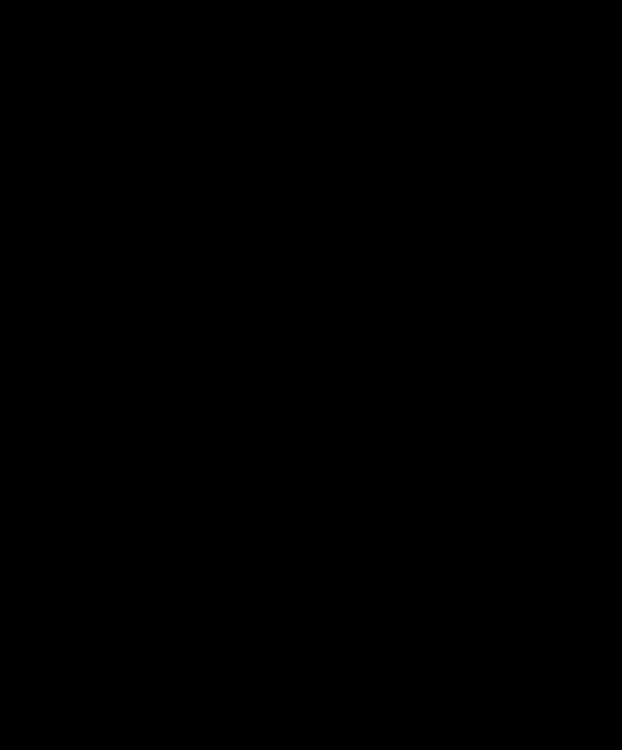
\includegraphics[width=0.7\textwidth]{fig/stochastic/overview_stochastic}
\caption{Stochastic Model in VOTCA. Overview of the different steps for generating stochastic charge transport networks in VOTCA. The Molecular Dynamics software GROMACS allows to analyze the radial distribution function of a morphology, which is then used by VOTCA::CSG to generate a coarse-grained potential that reproduces this distribution function. This potential can then be used for coarse-grained simulations in GROMCAS. For calculating rates in the coarse-grained morpholgy, first the relavant parameters are extracted (panalyze, eanalyze, ianalyze) from the reference morphology and and then reproduced in the coarsed-coarse grained morphology (neighborlist, eimport, iimport). With all these at hand, the rates calculator can be used in the coarse-grained morphology.}
\label{fig:overview_stochastic}
\end{figure*}

\subsection{Coarse-grained morphology}
The first step is to generate a coarse-grained morphology. In this example, it is done by mapping a DPBIC molecule (which consists of 103 atoms) to a single point, its center of mass and by using the iterative Boltzmann inversion (IBI) method. Starting point is a smaller reference morphology, generated with GROMACS. Using the command

\texttt{g\_rdf -f traj.xtc -s topol.tpr}

you can extract the radial distribution function $g(r)$ of your reference topolgy, outputted into the file rdf.xvg. This file, together with table.xvg,grompp.mdp, topol.top, index.ndx and confout.gro form your reference data.

For VOTCA::CSG you need a \textbf{setting.xml} file:

\lstset{language=XML2}
\begin{lstlisting}
<cg>
 <!-- example for a non-bonded interaction entry -->
 <non-bonded>
  <!-- name of the interaction -->
  <name>IR-IR</name>
  <!-- types involved in this interaction -->
  <type1>IR</type1>
  <type2>IR</type2>
  <!-- dimension + grid spacing of tables for calculations -->
  <min>0.5</min>
  <max>5.0</max>
  <step>0.01</step>
  <inverse>
   <!-- target distribution (rdf), just give gromacs rdf.xvg -->
   <target>rdf.xvg</target>
   <!-- update cycles -->
   <do_potential>1</do_potential>
   <!-- additional post processing of dU before added to potential -->
   <post_update>scale smooth</post_update>
   <post_update_options>
          <scale>0.5</scale> <!--Scale the potential before updating it -->
   	<smooth>
        	<iterations>2</iterations>
   	</smooth>
   </post_update_options>
   <!-- additional post processing of U after dU added to potential -->
   <post_add></post_add>
   <!-- name of the table for gromacs run -->
   <gromacs>
    <table>table_IR_IR.xvg</table>
   </gromacs>
  </inverse>
 </non-bonded>
   
 <!-- general options for inverse script -->
 <inverse>
  <!-- 300*0.00831451 gromacs units -->
  <kBT>2.49435300</kBT>
  <initial_configuration>maindir</initial_configuration>
  <!-- use gromacs as simulation program -->
  <program>gromacs</program>
  <!-- gromacs specific options -->
  <gromacs>
     <!-- trash so many frames at the beginning -->
     <equi_time>500</equi_time>
     <!-- grid for table*.xvg !-->
     <table_bins>0.001</table_bins>
     <!-- cut the potential at this value (gromacs bug) -->
     <pot_max>1000000</pot_max>
     <!-- extend the tables to this value -->
     <table_end>6.0</table_end>
  </gromacs>
  <!-- these files are copied for each new run -->
  <filelist>grompp.mdp topol.top index.ndx table.xvg</filelist>
  <!-- do so many iterations -->
  <iterations_max>500</iterations_max>
  <!-- Try to clean a bit -->
  <cleanlist>traj.xtc</cleanlist>
  <!-- ibm: inverse boltzmann imc: inverse monte carlo -->
  <method>ibi</method>
  <!-- write log to this file -->
  <log_file>inverse.log</log_file>
  <!-- write restart step to this file -->
  <restart_file>restart_points.log</restart_file>
  <!-- imc specific stuff -->
 </inverse>
</cg>
\end{lstlisting}

You run IBI using the command

\texttt{csg\_inverse --options settings.xml}

IBI intents to find a pontential $U(r)$ that reproduces your radial distribution function. It is stored in the file \textbf{table\_IR\_IR.xvg} in our example.

With the interaction potential at hand, a large topology can be generated using molecular dynamics simulations for the coarse grained model. Starting point is a box with equally distributed points, with each point representing one molecule and with the number of points chosen such that the density of the reference system is reproduced. A small python script can generate the conf.gro to start from, here shown to obtain a $50\times50\times120~{\rm nm}^3$ starting morphology.

\lstset{language=Python}
\begin{lstlisting}

from pylab import *
import numpy as np

lenX      =  50
lenY      =  50 
lenZ      =  120 
originalV = 4704.339 
originalN = 4000
spacing   = (originalV/originalN)**(1./3.) 

molecule  = "DPBIC"
resname   = "IRI"
atomname  = "IR"

newV = lenX*lenY*lenZ
newN = int(newV/originalV*originalN)

nX   = int(lenX/spacing)+1
nY   = int(lenY/spacing)+1
nZ   = int(lenZ/spacing)+1

print "max. molecules in X direction:  "+str(nX)
print "max. molecules in Y direction:  "+str(nY)
print "max. molecules in Z direction:  "+str(nZ)
print "total number of molecules: "+str(newN)

file = open("box.gro", "w")
file.write(molecule+"\n")
file.write(str(newN)+"\n")

atomnumber = 1
for iX in range(nX):
    for iY in range(nY):
        for iZ in range(nZ):
            if(atomnumber > newN):
                break
            posX = spacing*iX
            posY = spacing*iY
            posZ = spacing*iZ
            print >> file, "%5d%-5s%5s%5d%8.3f%8.3f%8.3f%8.4f%8.4f%8.4f" % \
            (1,resname,atomname,1,posX,posY,posZ,0,0,0)
            atomnumber += 1


file.write("  "+str(lenX)+"  "+str(lenY)+"  "+str(lenZ))
file.close()

print "Note: for some obscure reason VMD will not be able to read this file\
properly unless you open it once in vi and save it."


\end{lstlisting}

Open the box.gro in vi and save it (\texttt{:wq}), afterwards you can have a look at it in VDM. Run your MD simulations using the \texttt{mdrun} command. In the end you can compare the radial distribution functions of your reference and coarse-grained system, as shown in figure \ref{fig:stochastic}(a) as an example.

\subsection{Charge transport network}

\begin{figure*}[ht]
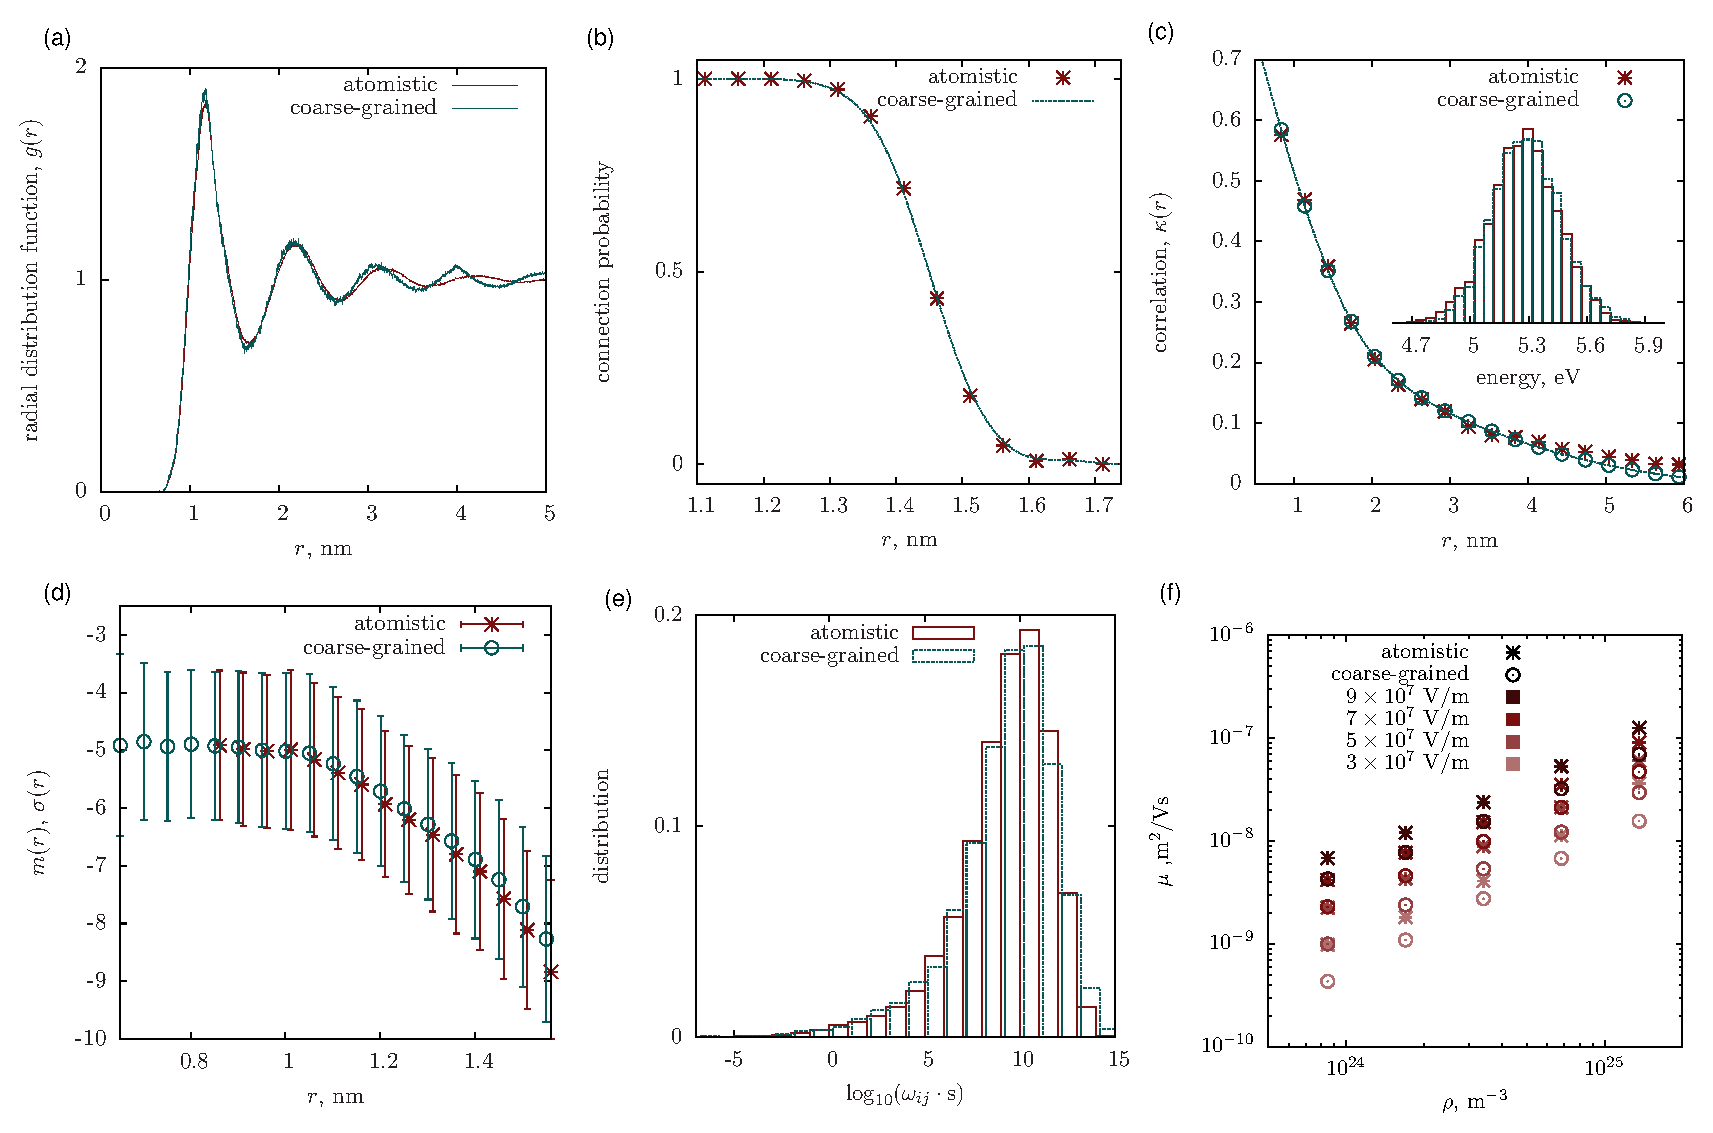
\includegraphics[width=1.0\textwidth]{fig/stochastic/stochastic}
\caption{ Comparison of the atomistic ($\unit[17\times17\times17]{nm^3}$) and coarse-grained ($\unit[50\times 50\times120]{nm^3}$) models. (a) Radial distribution function, $g(r)$. (b) Probability of two sites to be connected (added to the neighbor list) as a function of their separation. (c) Spatial site energy autocorrelation function, $\kappa(r)$; Inset:  Site energy distribution. (d) Mean $m$ and width $\sigma$ of a distribution of the logarithm of electronic couplings, $\log_{10}(\unit[J^2/]{eV^2})$, for molecules at a fixed separation $r$. (e) Rate distributions. (f) Mobility as a function of hole density, plotted for four different electric fields.}
\label{fig:stochastic}
\end{figure*}

To generate a charge transport network you first need a reference system with neighbor list, site energies and transfer integrals calculated and stored in a \textbf{state.sql} state file. The procedure for all these three properties is always the same: first analyze the reference data, and second import the analyzation files and reproduce the properties.




\subsubsection{Neighbor list}

In the atomistic reference system molecules are connected if their two closest segments are below a certain cut-off radius. This finer picture of segments does not exist in the coarse-grained system, where each molecule is represented by a point. To mimick the neighbor list, the probability of two molecules to be connected is analyzed as a function of their center-of-mass distance. This can be done by using the \emph{panalyze} calculator

\votcacommand{Analyze the pair connectivity (neighborlist) in the reference system}{\cmdpanalyze}

with the options defined as follows:
\\

\textbf{options\_analyze.xml}

\lstset{language=XML2}
\begin{lstlisting}
<options>
        <panalyze>
                <resolution_space>0.05</resolution_space>
        </panalyze>
</options>
\end{lstlisting}

The only parameter needed is the spacial resolution, i.e., the bin size for calculating the probabilities. The \emph{panalyze} calculator outputs a file \textbf{panalyze.distanceprobability.out} with the respective probabilities.
Now this file has to be imported into the coarse-grained state file

\votcacommand{Import the reference pair connectivity (neighborlist) and reproduce it in stochastic network}{\cmdnblst}

using the following options:
\\

\textbf{options\_import.xml}

\lstset{language=XML2}
\begin{lstlisting}
<options>
	<neighborlist>
                <probabilityfile>panalyze.distanceprobability.out</probabilityfile>
	</neighborlist>
</options>
\end{lstlisting}

For testing purposes, you can run the \emph{panalyze} calculator on your coarse-grained state file and compare the probability function to the reference. An example is shown in figure \ref{fig:stochastic}(b). You can also also look at the file \textbf{panalyze.distanceprobability.out} for both state files, which has the distribution of coordination numbers (number of neighbors) and its average in.

\subsubsection{Site energies}

Site energies in amorphous organic semiconductors are roughly Gaussian distributed, with the width of the Gaussian, $\sigma$, called the energetic disorder. However, there are correlations between sites if they are close enough to each other. The aim in this section is therefore to reproduce the correlated energetic landscape.
The first step is to get a spatial correlation function as well as the mean energy and the energetic disorder from your reference state file:
\\
\votcacommand{Analyze the energy distribution and correlation in the reference system}{\cmdeanast}

with the following options:
\\

\textbf{options\_analyze.xml}

\lstset{language=XML2}
\begin{lstlisting}
<options>
        <eanalyze>
                <resolution_sites>0.05</resolution_sites>
                <resolution_pairs>0.05</resolution_pairs>
                <resolution_space>0.3</resolution_space>
                <states>1,-1</states> <!-- +1 for hole transport, -1 for electron transport -->
                <distancemode>centreofmass</distancemode>
        </eanalyze>
</options>
\end{lstlisting}

The first three parameters determine bin sizes, then you can choose to look at hole and/or electron energy. The keyword \emph{centreofmass} means, that the correlation function is calculated as a function of the centre-of-mass distance of molecules and not as a function of their nearest segments. For the stochastic simulations you always have to use the \emph{centreofmass} mode!

The output files of this calculator that we need are \textbf{eanalyze.sitecorr\_e.out} (for electrons) and \textbf{eanalyze.sitecorr\_h.out} (for holes). In the second line of this file, you find mean and sigma of the energy distribution, as well as the mean of the static energies (without induction):
\\

\texttt{\# EANALYZE: SPATIAL SITE-ENERGY CORRELATION\\
\# AVG -0.4412655 STD 0.1739638 MIN\_R 0.8365040 MAX\_R 14.4771496  AVGESTATIC -0.4730655\\
...}
\\
These values have to be inserted manually into the options file for importing to the coarse-grained system (see below). Apart from that, the file contains the spatial correlation function.\\

You generate energies following this distribution and correlation by using the \emph{eimport} calculator

\votcacommand{Import the energy distribution and correlation and reproduce it in stochastic network}{\cmdeimport}

with the options:\\

\textbf{options\_import.xml}

\lstset{language=XML2}
\begin{lstlisting}
<options>
	<eimport>
                <probabilityfile_h>reference/eanalyze.sitecorr_h.out</probabilityfile_h>
                <sigma_h>0.1763163</sigma_h>
                <avgestatic_h>-0.5913265</avgestatic_h>
                <probabilityfile_e>reference/eanalyze.sitecorr_e.out</probabilityfile_e>
                <sigma_e>0.1739638</sigma_e>
                <avgestatic_e>-0.4730655</avgestatic_e>
                <cutoff>8.5</cutoff>
                <seed>1</seed>
	</eimport>
</options>
\end{lstlisting}

The \emph{cutoff} keyword can be used to read in the correlation function only up to a certain distance, which can be useful if larger distances yield unphysical results.

\subsubsection{Transfer Integrals}

The last ingredient reproduced by the stochastic approach are transfer integrals $J$. The idea is that $\log_{10}(\unit[J^2/]{eV^2})$ is roughly Gaussian distributed, with mean and error of the distribution varying with distance (see figure \ref{fig:stochastic} (d)). Use the calculator\\
\votcacommand{Analyze the distance-depend distribution of transfer integrals in the reference system}{\cmdianalyze}

with options\\

\textbf{options\_analyze.xml}

\lstset{language=XML2}
\begin{lstlisting}
<options>
        <ianalyze>
                <resolution_logJ2>0.05</resolution_logJ2>
                <resolution_space>0.05</resolution_space>
                <states>1,-1</states> <!-- +1 for hole transport, -1 for electron transport -->
        </ianalyze>
</options>
\end{lstlisting}

That will generate the files \textbf{ianalyze.ispatial\_e.out} and \textbf{ianalyze.ispatial\_h.out}, which contain means and errors as a function of centre-of-mass distance.\\

Now use the \emph{iimport} calculator to generate transfer integrals in the coarse grained state file, following the same statistics.

\votcacommand{Import distance dependent distribution of transfer integrals and reproduce in stochastic network}{\cmdiimport}


\textbf{options\_import.xml}

\lstset{language=XML2}
\begin{lstlisting}
<options>
	<iimport>
		<TI_tag></TI_tag>
		<TI_file></TI_file>
                <idft_jobs_file></idft_jobs_file>
                <probabilityfile_h>reference/ianalyze.ispatial_h.out</probabilityfile_h>
                <probabilityfile_e>reference/ianalyze.ispatial_e.out</probabilityfile_e>
	</iimport>
</options>
\end{lstlisting}

\subsubsection{einternal}
Run the \emph{einternal} calculator, just as you do it for the reference system.

\subsubsection{Rates}
If you followed the steps is this section, you have everything at hand to calculate charge transfer rates for the coarse grained system from the stochastic ingredients:

\votcacommand{Calculate rates in the stocchastic network}{\cmdratesst}

Options are the same as for the reference file. You can check the result by comparing rates from your reference to the coarse-grained system, see figure \ref{fig:stochastic}(e) for an example. The resulting charge transport network can be used for kinetic Monte Carlo simulations with VOTCA. If everything goes well, mobilities for both systems should agree, as shown in figure \ref{fig:stochastic}(f).

\section{Macroscopic observables}
\label{sec:analysis}%
Spatial distributions of charge and current densities can provide a better 
insight in the microscopic mechanisms of charge transport.
%
If $O$ is an observable which has a value $O_\alpha$ in a state $\alpha$, its 
ensemble average at time $t$ is a sum over all states weighted by the 
probability $P_\alpha$ to be in a state $\alpha$ at time $t$
%
\begin{equation}
\label{equ:ensemble}
\left< O \right> = \sum_{\alpha} O_\alpha P_\alpha.
\end{equation}
%
If $O$ does not explicitly depend on time, the time evolution of $\left< O 
\right>$ can be calculated as
\begin{equation}
\begin{split}
\frac{d \left< O \right>}{dt} = \sum_{ \alpha, \beta} 
      \left[ P_\beta \Omega_{\beta \alpha} - 
       P_\alpha \Omega_{\alpha \beta} \right] 
      O_\alpha %\\
 %     
      = \sum_{ \alpha, \beta} 
      P_\beta \Omega_{\beta \alpha}  
      \left[ O_\alpha - O_\beta \right] .
\end{split}
\end{equation}
%
If averages are obtained from KMC trajectories, $P_\alpha = s_\alpha / s$, where 
$s_\alpha$ is the number of Markov chains ending in the state $\alpha$ after 
time $t$, and $s$ is the total number of chains.

Alternatively, one can calculate time averages by analyzing a single Markov 
chain. If the total occupation time of the state $\alpha$ is $\tau_\alpha$ then
\begin{align}
\label{equ:time}
\overline{ O } 
= \frac{1}{\tau} \sum_{\alpha} O_\alpha \tau_\alpha \,,
\end{align}
where $\tau = \sum_{\alpha} \tau_\alpha$ is the total time used for time 
averaging.

For ergodic systems and sufficient sampling times, ensemble and time averages 
should give identical results. 
In many cases, the averaging procedure reflects a specific experimental 
technique. For example, an ensemble average over several KMC trajectories with 
different starting conditions corresponds to averaging over injected charge 
carriers in a time-of-flight experiment.  In what follows, we focus on the 
single charge carrier (low concentration of charges) case. 

\subsection{Charge density}
\label{sec:occupation}

For a specific type of particles, the microscopic charge density of a site $i$ 
is proportional to the occupation probability of the site, $p_i$
\begin{equation}
 \rho_i = e p_i / V_i\, ,
\end{equation}
where,  for an irregular lattice, the effective volume $V_i$ can be obtained 
from a Voronoi tessellation of space. For reasonably uniform lattices (uniform 
site densities) this volume is almost independent of the site and a constant 
volume per cite, $V_i = V/N$, can be assumed.  In the macroscopic limit, the 
charge density can be calculated using a sxtpthing kernel function, i.e. a 
distance-weighted average over multiple sites. Site occupations $p_i$ can be 
obtained from \equ{ensemble} or  \equ{time} by using the occupation of site $i$ 
in state $\alpha$ as an observable.

If the system is in thermodynamic equilibrium, that is without sources or sinks 
and without circular currents (and therefore no net flux) a condition, known as 
detailed balance, holds
%
\begin{equation}
\label{equ:detailed_balance}
  p_j \omega_{ji} = p_i \omega_{ij},
\end{equation}
%
It can be used to test whether the system is ergodic or not by correlating $\log 
p_i$ and the site energy $E_i$. Indeed, if $\lambda_{ij} = \lambda_{ji}$ the 
ratios of forward and backward rates are determined solely by the energetic 
disorder, $\omega_{ji} / \omega_{ij} = \exp(-\Delta E_{ij} / k_\text{B} T)$ (see 
\equ{marcus}).

\subsection{Current}
\label{sec:vaverage}
\index{current}
If the position of the charge, $\vec{r}$, is an observable, the time evolution 
of its average $\left<\vec{r}\right>$ is the total current in the system
\begin{equation}
 \vec{J} = e \left< \vec{v} \right> = e \frac{d \left< \vec{r}
   \right>} {dt} = e \sum_{i, j} p_{j} \omega_{ji} ( \vec{r}_i -
 \vec{r}_j ) .
\label{equ:current_def}
\end{equation}
Symmetrizing this expression we obtain
\begin{equation}
  \vec{J} = \frac{1}{2} e \sum_{i, j} \left( p_{j} 
  \omega_{ji} - p_{i} \omega_{ij} \right) \vec{r}_{ij} ,
 \label{equ:current}
\end{equation}
where $\vec{r}_{ij} = \vec{r}_{i} - \vec{r}_{j}$. Symmetrization ensures equal 
flux
splitting between neighboring sites and absence of local average fluxes in 
equilibrium. It allows to define a local current through site $i$ 
as\index{current!local}
\begin{equation}
  \vec{J_i} = \frac{1}{2} e \sum_{ j} \left( p_{j}  \omega_{ji} - p_{i} 
\omega_{ij} \right) \vec{r}_{ij} .
 \label{equ:site_current}
\end{equation}
A large value of the local current indicates that the site contributes 
considerably to the total current. A collection of such sites thus represents 
most favorable charge pathways~\cite{van_der_holst_modeling_2009}.

\subsection{Mobility and diffusion constant}
\label{sec:mobility}
\index{mobility}
For a single particle, e.g. a charge or an exciton, a zero-field mobility can be 
determined by studying particle diffusion in the absence of external fields. 
Using the particle displacement squared, $\Delta {\bm r}_i^2$, as an observable  
we obtain
 \begin{equation}
\begin{split}
2d D_{\gamma \delta} =  \frac{d \left<  \Delta{r}_{i, \gamma} \Delta{r}_{i, 
\delta} \right>}{dt} 
= \sum_{\substack{i,j \\ i\ne j}} p_j\omega_{ji} 
 \left( \Delta r_{i,\gamma}\Delta r_{i,\delta} - \Delta r_{j,\gamma}\Delta 
r_{j,\delta} \right)  
= \sum_{\substack{i,j\\ i\ne j}} p_j \omega_{ji} \left( r_{i,\gamma} 
r_{i,\delta} - r_{j,\gamma} r_{j,\delta} \right) \, .
\end{split}
\label{equ:diffusion}
\end{equation}
Here $\vec{r}_i$ is the coordinate of the site $i$, $D_{\gamma \delta}$ is the 
diffusion tensor, $\gamma, \delta = x,y,z$, and $d=3$ is the system dimension. 
Using the Einstein relation, 
\begin{equation}
 D_{\gamma \delta} = k_\text{B}T \mu_{\gamma \delta} \, ,
\end{equation}
one can, in principle, obtain the zero-field mobility tensor $\mu_{\gamma 
\delta}$. \Equ{diffusion}, however, does not take into account the use of 
periodic boundary conditions when simulating charge dynamics. In this case, the 
simulated occupation probabilities can be compared to the solution of the 
Smoluchowski equation with periodic boundary conditions  (see the supporting 
information for details). 

Alternatively, one can directly analyze time-evolution of the KMC trajectory and 
obtain the diffusion tensor from a linear fit to the mean square displacement, 
$\overline{ \Delta{r}_{i, \gamma} \Delta{r}_{i, \delta}} = 2d D_{\gamma \delta} 
t$. 

The charge carrier mobility tensor, $\hat{\mu}$, for any value of the external 
field can be determined either from the average charge velocity defined in
\equ{current_def} 
\begin{equation}
%\begin{split}
 \langle \vec{v} \rangle =  \sum_{i,j}  p_j  \omega_{ji}  (\vec{r}_i - 
\vec{r}_j) = \hat{\mu} \vec{F} \, ,
%\end{split}
\end{equation}
or directly from the KMC trajectory. In the latter case the velocity is 
calculated from the unwrapped (if periodic boundary conditions are used) charge 
displacement vector divided by the total simulation time. Projecting this 
velocity on the direction of the field $\vec{F}$ yields the charge carrier 
mobility in this particular direction. In order to improve statistics, 
mobilities can be averaged over several KMC trajectories and MD snapshots.

\subsection{Spatial correlations of energetic disorder}
\label{sec:eanalyze}

\index{site energy!spatial correlation}
Long-range, e.g. electrostatic and polarization, interactions often result in spatially correlated disorder~\cite{dunlap_charge-dipole_1996}, which affects the onset of the mobility-field (Poole-Frenkel) dependence~\cite{derrida_velocity_1983,novikov_essential_1998,nagata_atomistic_2008}.    

To quantify the degree of correlation, one can calculate the spatial correlation function of $E_i$ and $E_j$ at a distance $r_{ij}$
\begin{equation}
\label{equ:cf}
C(r_{ij}) = \frac{  \langle \left( E_i-\langle E\rangle \right)
                   \left( E_j-\langle E\rangle \right)\rangle}
                   {\langle\left( E_i -\langle E\rangle \right)^2\rangle},
\end{equation}
where $\langle E\rangle$ is the average site energy. $C(r_{ij})$ is zero if $E_i$ and $E_j$ are uncorrelated and $1$ if they are fully correlated. For a system of randomly oriented point dipoles, the correlation function decays as $1/r$ at large distances~\cite{novikov_cluster_1995}.

For systems with spatial correlations, variations in site energy differences, $\Delta E_{ij}$, of pairs of molecules from the neighbor list are smaller than variations in site energies, $E_i$, of all individual molecules. Since only neighbor list pairs affect transport, the distribution of $\Delta E_{ij}$ rather than that of individual site energies, $E_i$, should be used to characterize energetic disorder.

Note that the \calc{eanalyze} calculator takes into account {\em all} contributions to the site energies 
\votcacommand{Analyze distribution and correlations of site energeies}{\cmdeana}


%\input{theory/idft}
\section{Random Facts}

This section is a collection of facts we discovered about xtp and ctp which should be included in the manual at some point, but lack proper background.



\subsection{xqmm}

The cutoffs used should not exceed the dimension of the cell, at least for a non orthogonal unit cell. XQMM throws an error if your cutoff is larger than the box, but it does not take the extension of the molecule into accout, so often you may still have overlap.

XQMMM takes the segment coordinates from the MPS\textunderscore Files so be vary careful which MPS\textunderscore File you put in.


\subsection{EWALD}


\begin{itemize}
\item Use pewald3d, as a calculator. I am not sure what the rest is for. All still use the ewald options. The shape factor massively influences the results. For bulk systems "none" is the option of choice. Other options are "xyslab", "sphere", "cube" but I do not know what they do.
\item The induction cutoff should hardly ever exceed 3nm, because the calculation is expensive
\item If you want to use induction, you befor have to run ewdbgpol calculator and specify polar\textunderscore top.bgp in the options file for ewald. All the other parameters should be the same in ewdbpol and pewald3d
\end{itemize}

\subsection{GW-BSE}

There is a wide range of different approximations for $GW$-BSE. Here I try to summarize common abbreviations and methods and explain what our code does. This is not complete and certainly has some mistakes in it. 



\begin{itemize}
 \item COHSEX: RPA is only calculated for $\omega=0$. This amounts to $\varepsilon(\vctr{r},\vctr{r'},\omega)=\varepsilon(\vctr{r},\vctr{r'})$. This is also called the static approximation to $GW$
 \item Plasmon Pole model; RPA is calculated moslty twice, once at $\omega=0$ and $\omega=\omega_0$ , then these values are used to fit an analytic model to interpolate $\varepsilon(\vctr{r},\vctr{r'},\omega)$.
 \item Imaginary frequency integration, $\varepsilon$ is numerically integrated along the Imaginary frequency axis. This is done because $\varepsilon$ is much smoother along the Imaginary axis and thus requires less functional evaluations. Afterwards $\varepsilon$ is extended to real frequencies via analytic continuation.  
\end{itemize}

The calculation of $GW$. In VOTCA we also have the \textbf{shift} option. This is commonly called a scissor operator. This allows you to shift the unoccuppied KS-orbitals up in energy, making the resulting spectrum closer to the $GW$ spectrum. This is often a better starting point for the self-consistent evaluations.

\begin{itemize}
 \item $G_0W_0$. $G$ and $\varepsilon$ are calculated once from DFT results. $W$ is evaluated once from that. Then energies $ \varepsilon_i^{GW}$ are corrected via:
 \begin{equation}
   \varepsilon_i^{GW}=\varepsilon_i^{KS}+Z_i\bra{\phi^{KS}_i} \Sigma(\varepsilon_i^{KS})-V_{xc} \ket{\phi^{KS}_i}
 \end{equation}
 
 This is not implemented in VOTCA, because $GW_0$ is nearly as fast. 
 
 \item $GW_0$. $\varepsilon$ is calculated once from DFT results. $W$ is evaluated once from that. Then $\Sigma$ is calculated. The resulting energies are fed back into $\Sigma$, until self-consistency is achieved. This is denoted \textbf{fixed} in VOTCA.
 \begin{equation}
   \varepsilon_i^{GW}=\varepsilon_i^{KS}+\bra{\phi^{KS}_i} \Sigma(\varepsilon_i^{GW})-V_{xc} \ket{\phi^{KS}_i}
 \end{equation} 
 
 
 \item $scQPGW$. As $GW_0$, but after $\varepsilon_i^{GW}$ are converged, these energies are used to recalculate  $\varepsilon$ and then $W$, this is repeated until self-consistency is achieved. This is denoted \textbf{iterate} in VOTCA. This converges the ``eigenvalues'' of QP particles but along the $\ket{\phi^{GW}}$ states
 
 \item $scGW$. As $scQPGW$ but instead of correcting only the energies, the full $Sigma$ matrix is calculated and the eigenvalue problem for the QP is set up and solved and the whole system is then self-consistently solved in $\ket{\phi^{GW}}$ states and not in   $\ket{\phi^{KS}}$. This fully converges the eigenvalues and eigenvectors of the QP particles in the space spanned by $\ket{\phi^{KS}}$, e.g. $\ket{\phi^{GW}}$ are linear combinations of $\ket{\phi^{KS}}$. This is reported to be unstable because the vertex corrections are important now. This is at the moment implemented in VOTCA.
 

\end{itemize}

The calculations in BSE

\begin{itemize}
 \item 
\end{itemize}



\chapter{Input and output files}
\label{sec:io}
\section{Atomistic topology}
\label{sec:atomistic}

If you are using \gromacs for generating atomistic configurations, it is 
possible to directly use the topology file provided by \gromacs 
(\texttt{topology.tpr}). In this case the \gromacs residue and atom names should 
be used to specify the \slink{xmlmap}{coarse-grained topology}. 

A custom topology can also be defined using an \xml file. Moreover, it s 
possible to partially overwrite the information provided in, for example, 
\gromacs topology file. We will illustrate how to create a custom topology file 
using . The structure of  together with atom type definitions, is 
shown in fig.~\ref{fig:dcv2t}. has two thiophene (THI) and two 
dicyanovinyl (NIT) residues. The pdb file which contains residue types, residue 
numbering, atom names, atom types, and atom coordinates is shown in 
listing~\ref{list:pdb}.

\begin{figure}[ht]
\centering
\includegraphics[width=\textwidth]{./fig/chemical_structure/dcv2t}
\caption{\small (a)  with atoms labelled according to 
\texttt{residue\_number:residue\_name:atom\_name}. 
There are four residues and two residue types: thiophene (THI) and dicyanovinyl 
(NIT). The corresponding pdb file is shown in listing~\ref{list:pdb}. 
Atom numbering is used to split conjugated segments on rigid fragments and to 
link atomistic ((b) from GROMACS topology) and quantum descriptions (c).}
\label{fig:dcv2t}
\end{figure}

\lstinputlisting[
  language=XML,
  basicstyle=\ttfamily\footnotesize,
  stringstyle=\ttfamily\footnotesize,
  showstringspaces=false,
  frame=lines,
  label=list:pdb, 
  morekeywords={HETATM,THI,NIT},
  caption={ pdb file of.}]%
{./input/dcv2t/dcv2t.pdb}
\vfill
\section{Mapping file}
\label{sec:xmlmap}
The mapping file (referred here as \xmlmap) is used by the program \xtpmap to 
convert an atomistic trajectory to a trajectory with conjugated segments and 
rigid fragments. 
This trajectory is stored in a \slink{statefile}{state file} and contains 
positions, names, types of atoms belonging to rigid fragments. 
The description of the mapping options is given in table \ref{tab:map}. An 
example of \xmlmap for a molecule is shown in listing~\ref{list:map}. 

The file \xmlmap contains the whole electrostatic information about the 
molecules as well as the structural information. The \tool{pdb2map} creates a 
\xmlmap from a pdb file and is a good starting point for further refinement. 
%
\begin{table}[h]
\label{tab:map}
\caption{Description of the \xml mapping file (\xmlmap).}
\rowcolors{1}{invisiblegray}{white} {\footnotesize 
\input{reference/xml/map.xml}}
\end{table}
%
% Define new language for listings.
\lstdefinelanguage{MXML} {
   basicstyle=\ttfamily\scriptsize,
   sensitive=true,
   morecomment=[s][\color{gray}\rmfamily\itshape]{<!--}{-->}, 
   showstringspaces=false,
   numberstyle=\scriptsize,
   numberblanklines=true,
   showspaces=false,
   breaklines=true,
   showtabs=false,
   alsoletter={:},
   keywords = [1]
   { 
topology,molecules,molecule,name,mdname,segments,segment,fragments,fragment,
mdatoms,qmatoms,localframe,weights},
   keywordstyle={[1]\color{blue}},
}

\lstinputlisting[
 language=MXML,
 label=list:map,
 caption={Examle of \xmlmap for. Each rigid fragment (coarse-grained bead) 
is defined by a list of atoms. Atom numbers, names, and residue names should 
correspond to those used in \gromacs topology (see the corresponing listing 
\ref{list:pdb} of the pdb file).}]%
{./input/dcv2t/map.xml}


%\section{Conjugated segments}
\label{sec:xmlsegments}
The file describing hopping sites, or conjugated segments, is used by practically all programs and calculators. It links the coarse-grained trajectory (positions and orientations of rigid fragments) and quantum-mechanical descriptions of all conjugated segments. The description of this \xml file (\xmlsegments) is given in table \ref{tab:segments}. An example for \dcvt is shown in listing~\ref{list:segments}.
%
\begin{table}[h]
\caption{Description of conjugated segments (\xmlsegments).} 
\label{tab:segments}
\rowcolors{1}{invisiblegray}{white} {\footnotesize \input{reference/xml/segments.xml} }
\end{table}
%
\lstdefinelanguage{MXML} {
   basicstyle=\ttfamily\scriptsize,
   sensitive=true,
   morecomment=[s][\color{gray}\rmfamily\itshape]{<!--}{-->}, 
   showstringspaces=false,
   numberstyle=\scriptsize,
   numberblanklines=true,
   showspaces=false,
   breaklines=true,
   showtabs=false,
   alsoletter={:},
   keywords = [1]
{segments,segment,coordinates,orbitals,basisset,torbital,reorg_charging,reorg_discharging,qneutral,qcharged,energy,beadconj,molname,name,map,weights},   
  keywordstyle={[1]\color{blue}},
}
%
\lstinputlisting[
 language=MXML,
 label=list:segments,
 caption={\small \xml file describing \slink{segments}{conjugated segments}. Note that the mapping and weights for each segment are separated by a colon. 
}]%
{./input/dcv2t/segments.xml}






\section{Monomer calculations for DFT transfer integrals}
\lstinputlisting[
  language=XML,
  label=list:edft_gaussian_xml,
  stringstyle=\ttfamily\footnotesize,
  showstringspaces=false,
  caption={\small Example {\tt package.xml} file for the \gaussian package required in the options of the \calc{edft} \calculator for the monomer calculations as preparation for the determination of transfer integrals using \dipro.}] {./input/qmpackage_headers/gaussian_edft.xml}

\lstinputlisting[
  language=XML,
  label=list:edft_turbomole_xml,
  stringstyle=\ttfamily\footnotesize,
  showstringspaces=false,
  caption={\small Example {\tt package.xml} file for the \turbomole package required in the options of the \calc{edft} \calculator for the monomer calculations as preparation for the determination of transfer integrals using \dipro.}] {./input/qmpackage_headers/turbomole_edft.xml}

\lstinputlisting[
  language=XML,
  label=list:edft_nwchem_xml,
  stringstyle=\ttfamily\footnotesize,
  showstringspaces=false,
  caption={\small Example {\tt package.xml} file for the \nwchem package required in the options of the \calc{edft} \calculator for the monomer calculations as preparation for the determination of transfer integrals using \dipro.}] {./input/qmpackage_headers/nwchem_edft.xml}
\section{Pair calculations for DFT transfer integrals}
\lstinputlisting[
  language=XML,
  label=list:idft_gaussian_xml,
  stringstyle=\ttfamily\footnotesize,
  showstringspaces=false,
  caption={\small Example {\tt package.xml} file for the \gaussian package required in the options of the \calc{idft} \calculator for the pair calculations and the determination of transfer integrals using \dipro.}] {./input/qmpackage_headers/gaussian_idft.xml}

\lstinputlisting[
  language=XML,
  label=list:idft_nwchem_xml,
  stringstyle=\ttfamily\footnotesize,
  showstringspaces=false,
  caption={\small Example {\tt package.xml} file for the \nwchem package required in the options of the \calc{idft} \calculator for the pair calculations and the determination of transfer integrals using \dipro.}] {./input/qmpackage_headers/nwchem_idft.xml}
\section{DFT transfer integrals}
\lstinputlisting[
  language=XML,
  label=list:TI_xml,
  stringstyle=\ttfamily\footnotesize,
  showstringspaces=false,
  caption={\small Example {\tt TI.xml} file created as the output of a \dipro calculation. Due to slightly different implementations, the orbitals indices refer to monomer indices in a \gaussian run but to indices in the merged dimer guess in a \turbomole run.}] {./input/TI.xml}


\section{State file}
\label{sec:statefile}
All data structures are saved to the \sqlstate file in sqlite3 format, see http://www.sqlite.org/.
They are available in form of tables in the \sqlstate file as can be seen by the command\\
{\small \sqlite \sqlstate \texttt{" .tables "}}

An example of such a table are \sqlmolecules. The full table can be displayed using the command (similar for the other tables)\\
{\small \sqlite \sqlstate \texttt{" SELECT * FROM \sqlmolecules"}}\\
The meaning of all the entries in the table can be displayed by a command like\\
{\small \sqlite \sqlstate \texttt{" .SCHEMA \sqlmolecules"}}\\
The first and second entry are  integers for internal and regular id of the molecule and the third entry is the name. 
A single field from the table like the name of the molecule can be displayed by a command like\\
{\small \sqlite \sqlstate \texttt{" SELECT name FROM \sqlmolecules"}}\\
Besides \sqlmolecules, the following tables are stored in the \sqlstate:

\sqlconjsegproperties:\\
Conjugated segments are stored with id, name and x,y,z coordinates of the center of mass in nm.

\sqlconjsegs:\\
Reorganization energies for charging or discharging a conjugated segment are stored together with the coulomb energy and any other user defined energy contribution (in eV) and occupation probabilities.

\sqlpairs:\\
The pairs from the neighborlist are stored with the pair id, the id of the first and second segment, the rate from the first to the second , the rate from the second to the first (both in s$^-1$)  and the x,y,z coordinates in nm of the distance between the first and the second segment.

\sqlpairintegrals:\\
Transfer integrals for all pairs are stored in the following way:  The pair id , the number for counting possible different electronic overlaps (e.g if only the frontier orbitals are taken into account this is always zero, while an effective value is stored in addition to the different overlaps of e.g. HOMO-1 and HOMO-1 if more frontier orbitals are taken into account) and the integral in eV.

\sqlpairproperties:\\
The outer sphere reorganization energy of all pairs is stored by an id, the pair id, a string \texttt{lambda\_outer} and the energy in eV.

\sqlconjsegs:\\
Conjugated segments are saved in the following way: The id, the name, the type, the molecule id, the time frame, the x,y,z coordinates in nm and the occupation probability.

\sqlconjsegproperties:\\
Properties of the conjugated segments like reorganization energies for charging or discharging a charge unit or the coulomb contribution to the site energy are stored by: id, conjugated segment id, a string like \texttt{lambda\_intra\_charging}, \texttt{lambda\_intra\_discharging} or \texttt{energy\_coulomb} and a corresponding value in eV.

The tables \sqlrigidfragproperties, \sqlrigidfrags and \sqlframes offer information about rigid fragments and time frames including periodic boundary conditions.


The data in the \sqlstate file can also be modified by the user. Here is an example how to modify the transfer integral between the conjugated segments number one and two assuming that they are in the neighborlist.
Their pair id can be found by the command \\ 
{\small \texttt{pair\_ID=`}\sqlite \sqlstate \texttt{"SELECT \_id FROM pairs WHERE conjseg1=1 AND conjseg2=2"`}} \\
The old value of the transfer integral can be deleted using\\
{\small \sqlite \sqlstate \texttt{"DELETE FROM pair\_integrals WHERE pair=\$pair\_ID"}}\\
Finally the new transfer integral $J$ can be written to the \sqlstate file by the command\\
{\small \sqlite \sqlstate \texttt{"INSERT INTO pair\_integrals (pair,num,J) VALUES (\$pair\_ID,0,\$J)"}}
Here the \texttt{num=0} indicates that only the effective transfer integrals is written to the file, while other values of \texttt{num}
would correspond to overlap between other orbitals than the frontier orbitals.

In a similar way the coulomb contribution to the site energy of the first conjugated segment can be overwritten by first getting its id\\
{\small \texttt{c\_ID=`}\sqlite \sqlstate \texttt{"SELECT \_id from conjseg\_properties}}
{\small \texttt{ where conjseg=1 AND key =$\backslash$"energy\_coulomb$\backslash$""}} \\
Then deleting the old value\\
{\small \sqlite \sqlstate \texttt{"DELETE FROM from conjseg\_properties WHERE \_id=\$c\_ID"}}\\
Then the new coulomb energy $E$ can be written to this id\\
{\small \sqlite \sqlstate \texttt{"INSERT INTO conjseg\_properties (\_id,conjseg,key,value)\\ 
VALUES (\$c\_ID,1,$\backslash$"energy\_coulomb$\backslash$",\$E)"}}\\
Finally the resulting coulomb contribution to all conjugated segments can be displayed by\\
{\small \sqlite \sqlstate \texttt{"SELECT * from conjseg\_properties WHERE key=$\backslash$"energy\_coulomb$\backslash$""}}


\chapter{Reference}
\label{sec:reference}
\section{Programs}
\label{ref:programs}
\label{sec:programs}
Programs execute specific tasks (calculators). 

\input{reference/programs/all}

\section{Calculators}
\label{ref:calculators}
\label{sec:calculators}

Calculator is a piece of code which computes specific system properties, such as site energies, transfer integrals, etc. \xtprun  are wrapper programs which executes such calculators. The generic syntax is 
\vskip 0.2cm
{\noindent \small \xtprun \exe \texttt{"calc1, calc2, ..."} \opt \xmloptions }
\vskip 0.2cm
%
File \xmloptions lists all options needed to run a specific calculator. The format of this file is explained in listing~\ref{list:calc}. A complete list of calculators is given in the \refcalc reference section.
%
\lstinputlisting[label=list:calc, 
 caption={\small A part of the \xmloptions file with options for the \texttt{calculator\_name\{1,2\}} \refcalc.
}]{./reference/calculators.xml}

A list of all calculators and their short descriptions can be obtain using 
\vskip 0.1cm
{\noindent \small \xtprun \texttt{-{}-list} }
\vskip 0.1cm

A detailed description of all options of a specific calculator(s) is available via
\vskip 0.1cm
{\noindent \small \xtprun \texttt{-{}-desc calc1,calc2,...} }

\input{reference/calculators/calculators}
\vfill

\section{Common options}
\label{ref:options}
%\setdefaultleftmargin{0.8em}{0.8em}{0.8em}{0.8em}{0.8em}{0.8em}
\rowcolors{1}{invisiblegray}{white}
{\small 
\input{reference/xml/options.xml}
}
\vfill




%\appendix
%\input{appendix/xtp_standalone}

\nolinenumbers

\bibliographystyle{short}
{\footnotesize \bibliography{xtp-manual} }

\end{document} 
